%Dissertation Template for Columbia University Ph.D. programs
%By Charles McNamara, 2016
%I posted this document under a CC0 public domain license -- do whatever you want with it!
%It's probably a good idea to review the university guidelines just so you know what you want your dissertation to look like. You can read about those guidelines at this site: http://gsas.columbia.edu/content/formatting-guidelines.
%Good luck writing your dissertation!




% This is the main document file for the dissertation. You should not include any of your actual chapters or other substantive writing in this file.
%First we have to set up the style and formatting of the pages.

\documentclass[letterpaper,12pt]{memoir} %The memoir class is great for longer works that use separate chapters. The Dissertation Office recommends 10-pt Arial or 12-pt Times New Roman. I use 12-pt for readability.


%%%%%%%%%%%%%%%%%%%%%%%%%%%%%%%%%%%%
%% packages from the switch paper %%
%%%%%%%%%%%%%%%%%%%%%%%%%%%%%%%%%%%%

%\usepackage[utf8]{inputenc}
\usepackage{array}
\usepackage{arydshln}
\setlength\dashlinedash{0.2pt}
\setlength\dashlinegap{1.5pt}
\setlength\arrayrulewidth{0.3pt}
\usepackage{booktabs}
\usepackage{float}
\usepackage{titlesec}
\usepackage{capt-of}
\usepackage{graphicx}
\usepackage{adjustbox}
\usepackage{soul}
\usepackage{siunitx}
\usepackage{upgreek}
\usepackage{csquotes}



%Below are some LaTeX packages to include to make sure that your Unicode characters render correctly. This is especially important if your dissertation includes polytonic Greek!

\RequireXeTeX %XeTeX allows you to use Unicode characters like polytonic Greek in your writing.
\usepackage{fontspec} %Allows you to load fonts in XeTeX.
\defaultfontfeatures{Mapping=tex-text} %Allows you to get pretty TeX ligatures in your writing.
\usepackage{xunicode} %You need this for Unicode fonts to work properly.
\usepackage{xltxtra} %Some extra font capabilities for XeTeX
\DisemulatePackage{setspace} %You need to use this package for "true MS Word" double-spacing.
\usepackage{setspace} %Allows you to set different spacing (double, etc.) throughout your writing.
% \usepackage{hyperref} % Use if you want hyperlinks in your table of contents

\setmainfont{Linux Libertine O} %This is a really readable serif font. It renders polytonic Greek better than any other OpenType font I've found, including Times New Roman. I now use it for everything, including class handouts. Highly recommended for classicists.

\usepackage{enumitem} % To fix spacing of bullet point lists
\setlist{noitemsep} % or \setlist{nosep} for space around whole list



%Here is some stuff on the bibliography. You want to keep your bibliography file in the same directory as this file.

\usepackage[american]{babel} %Enables hyphenation and date formats according to American conventions. Change "american" to "british" (or another value) if you work outside the US.
%\usepackage[backend=bibtex8,style=authoryear-icomp,texencoding=utf8,bibencoding=utf8]{biblatex} 


%\usepackage[backend=bibtex8,style=numeric,texencoding=utf8,bibencoding=utf8]{biblatex} 

\usepackage[natbib=true,style=numeric,sorting=none]{biblatex}
%\usepackage[sectionbib]{chapterbib}
%\usepackage[numbers,sort&compress]{natbib}


%The command here uses biblatex to render your bibliography, and it tells biblatex to use Unicode fonts. You can change the style of your citations easily by changing the value for "style" -- I use authoryear-icomp which takes care of the id/ibid citations automatically. There are many styles available if you want to change it.
%I have tried to use biber instead of biblatex many times, but it's never worked properly for me. I use biblatex, but feel free to try biber instead. 
\addbibresource{./Bibliography_CH2.bib} 
\addbibresource{./Bibliography_CH3.bib} 
\addbibresource{./Bibliography_CH5.bib}

%Your bibliography file. I use JabRef to keep track of my bibliography. Highly recommended, and free! You can use Zotero if you want, but I've had trouble exporting to .bib files from my Zotero database.
\setlength{\bibitemsep}{\baselineskip} %Skip lines between bibliography entries. Columbia requires that you skip a line between entries.



%Here you can set margins and other page formatting

\setlrmarginsandblock{3.175cm}{3.175cm}{*} %Left and right margin -- the dissertation office requires at least 1-inch margins
\setulmarginsandblock{2.54cm}{2.54cm}{*}  %Upper and lower margin -- same thing, at least 1-inch margins
\checkandfixthelayout %A function of the memoir class that finds the right number of lines per page and apparently tidies up the formatting in other mysterious ways...?




% Below we start to set up the document itself, including how to use spacing throughout the dissertation.

\begin{document}

\sloppy %If I don't include sloppy, then Greek and Latin words screw up margins all over. If you don't include weird languages in your dissertation, you can probably leave this one out.
\chapterstyle{chappell} % Nice formatting for chapter headings. Check out the documentation for the memoir class for other options.
\footnotesep\baselineskip % Footnotes need to have a space between each one for Columbia's Dissertation Office. 
\setstretch{2} %Set line spacing to "true MS Word" double-spacing
%\DoubleSpace % Use LaTeX double-spacing (more like 1.666 spacing)

\expandafter\def\expandafter\quote\expandafter{\quote\SingleSpace} %Keep all block quotes single-spaced regardless of body text spacing.
\pagestyle{plain} %Put page numbers at the bottom-center for the whole dissertation. Columbia's dissertation office requires that the numbers appear at this location on the page throughout the document.



%% Here's the Title Page
% This is the title page of my dissertation.
% You may need to change the text on this page for your particular department. Consult the Dissertation Office Formatting Guidelines.

\thispagestyle{empty} % No page number
\begin{center}
  \SingleSpace

  \vspace*{1in}

 Silicon Photonic Subsystems for Optically Reconfigurable and Disaggregated Memory Access

  \bigskip % Get space between title and author name

  Alexander Gazman

  \vspace{5in}

  Submitted in partial fulfillment of the\\
  requirements for the degree of\\
  Doctor of Philosophy\\
  in the Graduate School of Arts and Sciences

  \bigskip
  \bigskip

  COLUMBIA UNIVERSITY

  \bigskip % Get space between Columbia and the year

  2019
\end{center}


%% Here's the copyright page. I use a Creative Commons license.
% This is the copyright page of my dissertation.
% You might also consider using a Creative Commons license. Ask your adviser or the university's Copyright Office.

\thispagestyle{empty} % No page number
\null\vfill % Pushes Copyright to the bottom of the page.
\begin{center}
  \SingleSpace %Keep the Copyright single-spaced
© 2019\\
Alexander Gazman\\
All rights reserved\\
\end{center}


%% Here's the Abstract
% This is the abstract of my dissertation.

\pagestyle{empty} % No page number in entire abstract
\begin{center}
  ABSTRACT

  Silicon Photonic Subsystems for Optically Reconfigurable and Disaggregated Primary Memory Access

  Alexander Gazman
\end{center}

Silicon Photonic technology has undergone a tremendous progress in the past decade. From demonstrations of integrated photonic designs consisting of several elements fabricated in academic and research institutes to complex designs consisting of hundreds of elements. This progress is attributed to the availability of mature and reliable semiconductors foundries such as AIM, IME, IMEC and Global Foundries. As in electrical CMOS design, these foundries provide PDKs that allow to integrate optical building blocks. These PDKs includes elements such as waveguides, Mach-Zehnder interferometers, ring resonators, passive splitters, photo-detectors and fiber coupling elements in order to design complex subsystems such as high-port count switches, transceivers and sensors. To utilize these design, the optical operation of these hundreds to elements needs to be 



consists of tenth to hundreds of optical elements that needs to be biased and simultaneously controlled to achieve an optimal operation. For system integration, the physical layer needs to be abstracted through a simple and closed-loop control plane. 

In this thesis, 



\frontmatter
\tableofcontents % You need to put your ToC after frontmatter so that it will get lowercase Roman numerals.

%A list of graphs and illustrations should go here if you use any.

% Acknowledgements
\include{./FrontMatter/Acknowledgments}

% Dedication
\include{./FrontMatter/Dedication}

% Preface if you have one




%What follows is the main text of your dissertation. You can comment out lines if you want to exclude them from your document for drafts. Everything after \mainmatter will get Arabic numbers centered on the bottom of the page.

\mainmatter

%I use subdirectories for each part of my dissertation just to keep the files tidy. LaTeX generates a lot of different files for output, and using subdirectories allows you to find your .tex files more easily.

%The following command starts your introduction. 

\chapter*{Introduction} %Your introduction isn't a numbered chapter, so we use the asterisk here.

\addcontentsline{toc}{chapter}{Introduction} %This command puts your introduction in your table of contents even though we have used the asterisk in the \chapter command above.

** What is Silicon Photonics
** The premise of Silicon - integration - io
** motivation - low cost, high volume 
** success in electronics to optical domain


Here you can write some introductory remarks about your chapter.
I like to give each sentence its own line.

When you need a new paragraph, just skip an extra line.

\section*{New Section}

By using the asterisk to start a new section, I keep the section from appearing in the table of contents.
If you want your sections to be numbered and to appear in the table of contents, remove the asterisk.


%This is the first chapter of the dissertation

%The following command starts your chapter. If you want different titles used in your ToC and at the top of the page throughout the chapter, you can specify those values here. Since Columbia doesn't want extra information in the headers and footers, the "Top of Page Title" value won't actually appear.
\pagestyle{plain}

\chapter[Silicon Photonic platform for optically connected memory][Top of Page Title]{Silicon Photonic platform for optically connected memory}

Here you can write some introductory remarks about your chapter.
I like to give each sentence its own line.

When you need a new paragraph, just skip an extra line.

\section{New Section}

By using the asterisk to start a new section, I keep the section from appearing in the table of contents.
If you want your sections to be numbered and to appear in the table of contents, remove the asterisk.


%This is the second chapter of the dissertation

%The following command starts your chapter. If you want different titles used in your ToC and at the top of the page throughout the chapter, you can specify those values here. Since Columbia doesn't want extra information in the headers and footers, the "Top of Page Title" value won't actually appear.
\pagestyle{plain}

\chapter[Controlling and Monitoring performance of large scale Silicon Photonic devices][Top of Page Title]{Controlling and Monitoring performance of large scale Silicon Photonic devices}

\textit{\textbf{Abstract - } In this chapter, we develop scalable solutions for controlling optical properties and in-line power monitoring of silicon photonic device. The first part of the chapter concerns with model development of the thermo-optic effect of integrated heaters. Building on the analytical models, we present a control scheme based on pulse-width modulation (PWM) signals to demonstrate a DAC-less resonance control in MRR. A study in the required PWM frequency is presented and experimentally measured to achieve a minimal ripples operation in the optical domain.}

\textit{The second part of the chapter is focused on doped heater elements, and their associated photo-conductance (PC) effect. Measuring the change of the heater conductance, enables to utilize this heater design for both controlling and optical power monitoring purposes. We show this mechanisms when doped heaters are integrated in micro-ring and Mach-Zehnder devices. The PC effect is experimentally characterized for the steady state and the transient response and compact models for the PC current are developed.}

\section{Introduction}

The Silicon Photonic platform provides a wide ranges of elements to support a variety of applications in high-speed optical communications. From coherent generation \cite{novack2018silicon} and switching \cite{vujicic2017software} to direct detection \cite{aoki2017low} links with total aggregated bandwidths in the order of Tbps. Theses designs consist of tenth to hundreds of integrated elements, and recent studies showed that these links can achieve an overall energy consumption below 2pJ/bit \cite{bahadori2016energy,bahadori2017energy} which is a highly desirable metric system performance. Achieving these highly efficient performances in practice requires that each element in the system is operated at its optimal conditions to overcome fabrication variations \cite{chrostowski2014impact} and compensated for thermal sensitivity \cite{padmaraju2014resolving}. 

As in electronics, where transistors are biased to a specific operational point, a similar principle holds with integrated photonic devices. For example, due to the narrow-band nature of the MRRs, when used as receivers or transmitter, their resonance must biased to the desired WDM channel \cite{bogaerts2012silicon}. Mach-Zehnder based modulators are biased to the linear point of the transfer function \cite{li2013any} and in a cascaded configurations when used as filters \cite{Guan_1xN,horst2013cascaded} or switches \cite{chen2016low} they are biased to the desired routing configuration. \textbf{can add more citations from the thermal paper}

The most common technique for biasing SiP elements is by means of precise control the local temperature of waveguide's section. Integrated micro-heating structures are fabricated using either metallic traces on top of the waveguide \textbf{atabaki2010optimization} or by doping the waveguide \cite{harris2014efficient}. When applying ohmic power in these heaters, the optical behavior is changed due to the high the thermo-optic coefficient in Silicon material \cite{komma2012thermo}. Effectively, by changing the index of refraction with thermal control, we manipulate the phase of the optical carrier in the thermal region []. 

Designs based on external heaters must take into account the fact that heat diffusion is not instantaneous -- it takes time for the heat to propagate from the heater to the waveguide. Moreover, the heat might reach the waveguide at different strengths and different delays.  The optical operation of the photonic device depends, therefore, on the frequencies of the electrical excitation signal applied to the heater. Understanding this transient thermal response is crucial to finely adjust and efficiently counter-balance the thermal noise that impacts the response of silicon photonic devices. 


%Current discussion of transient thermal response is reduced to experimental considerations, specifically a posteriori characterizations of rise and fall times (the time required for the temperature of the waveguide to evolve from 10\% to 90\% and 90\% to 10\% of its asymptotic values, respectively), while the stationary thermal response is straightforward to model accurately \cite{wang2017fast}.  Observing the importance of thermal stabilization in the total power budget of a photonic link \cite{bahadori2017energy}, we conclude that the understanding of thermal effects in silicon photonics platform deserves careful study 

The first goal of this chapter is to provide a comprehensive analysis and models for the thermo-optic effects in the SiP platform. Then we study how thermal variations affecting temperature-dependent devices can be adequately rectified with digitally driven signals. In particular, we look at thermal tuning using pulse width modulation (PWM) signals generated by relatively simple digital logic \cite{matsuura2017accelerating, zecevic2015integrated, aguinaldo2014wideband}. 

Our motivation for investigating PWM control is due to the fact that as the number of active SiP devices increases and reach hundred to thousands elements in integrated photonic applications []. The use of traditional digital-to-analog converters (DACs) in heterogeneous integration can be problematic to support such a high number of elements. As an alternative, a single FPGA with large number of I/Os can supports such systems. Additionally, the use of PWM control paradigm, the total power consumption of the driving circuitry can be further reduced comparing to constant voltage solutions \cite{zecevic2015integrated}. 

The second goal of this chapter is utilizing photo-conductance (PC) effect in silicon photonic doped thermo-optic phase-shifter (waveguide-doped heaters) \cite{Harris_heater}. As the optical signal (continuous or modulated) propagates through this heater design, the interaction between photons and impurities in the doped silicon generates free electrical carriers \cite{jayatilleka2019photoconductive}. As a result, the conductance of the heater is increasing proportionally with the optical power. We characterize the PC effect in MRR and MZI based designs, and develop a compact model for the photo-conductance current. 

From a system prospective, this functionality is highly desirable since it enables utilizing doped heaters as both controlling and \textit{in-line} power monitoring elements. Furthermore, it can greatly reduce design complexity which does not require tapping the signal for monitoring purposes[], reduce the total footprint area, and the number of I/O in closed-loop solutions [].

\section{Integrated Heater and Waveguide System}

By applying an electrical control to the integrated heater element, we locally change the temperature of a waveguide section. The temperature change affects the effective index of refraction of the waveguide, and as a result adjusting the phase of the propagating optical signal. The is described by the following equation:

\begin{equation}
\label{CH3_eq1}
     \Delta n_\text{eff} \approx dn_\text{eff}/dT \times \Delta T.
\end{equation}

where the thermo-optic sensitivity of a silicon waveguide surounded by a silica waveguide $dn_\text{eff}/dT$ =  2.1$\times$10$^{-4}$ K$^{-1}$. 

A schematic of the waveguide and a heater system is shown in Fig. \ref{CH3_fig2}(a). A strip waveguide with a micro-heater situated at a distance $d$. By applying a voltage to the heater, $V(t)$, the corresponded current is, $I(t)$, and the total dissipated ohmic power is $P(t)$ = $V(t)\times I(t)$ that causes the waveguide temperature to rise ($\Delta T_H$). To develop an expression

We are interested in expressing the temperature rise $\Delta T_H$ as a function of the applied voltage $V(t)$. We first note that would the resistance of the heater $R$ stay constant, the power dissipated would be strictly a quadratic function of the voltage as $I(t)$ = $V(t)/R$ and thus $P(t)$ = $V^2 (t)/R$. However, as the heater temperature increases, the resistivity of the heater increases according to $R$ = $R_\text{linear} (1 + \alpha_H \Delta T_H$) where $\alpha_H$ is the temperature coefficient of the resistance of the heater ($\alpha_H \sim 3\times 10^{-3}-8\times 10^{-3}$ K$^{-1}$ for most metals). The increased resistivity leads in turn to a decrease of the current and dissipated ohmic power. The self-heating situation of the heater finally regulates itself at a steady sate of temperature and supplied current. We assume that the self-heating of heater is instantaneous, i.e. the resistivity of the heater instantaneously changes with a change in the applied voltage. As further detailed in Appendix I, the temperature of heater linearly depends on the dissipated ohmic power where the proportionality coefficient is considered to be constant over time. The temperature of heater then follows the voltage of heater according to
%
\begin{equation}\label{CH3_eq2}
\Delta T_H = \frac{1}{2\alpha_H}\left(-1+\sqrt{1 + K_v V^2 (t)}\right)
\end{equation}
%
where $K_v$ represents the thermal nonlinearity of the ohmic resistance. The result of such self-heating phenomenon is a nonlinear DC voltage-current characteristic of the resistive heater given by
%
\begin{equation}\label{CH3_eq3}
I(t) = \frac{V(t)}{R_\text{linear}}\times \frac{2}{1+\sqrt{1 + K_v V^2 (t)}} .
\end{equation}
%
Note that if $\alpha_H \rightarrow 0$ then $K_v \rightarrow 0$, and Eq. (\ref{eq1}) and (\ref{eq2}) reduce to the simple forms for a linear resistance. 
Fig. \ref{fig2}(b) shows an example of experimentally measured V-I data points (blue circles) along with an expected linear V-I curve (dashed red line). By fitting Eq. (\ref{eq2}) to the measured data points, we find out that with parameters $R_\text{linear}$ = 161 $\Omega$ and $K_v$ = 0.6 V$^{-2}$, the model matches the measurements quite well. Fig. \ref{fig2}(c) schematically depicts the heat distribution after the self-heating of heater is reached.







\begin{figure}[t]
\begin{center}
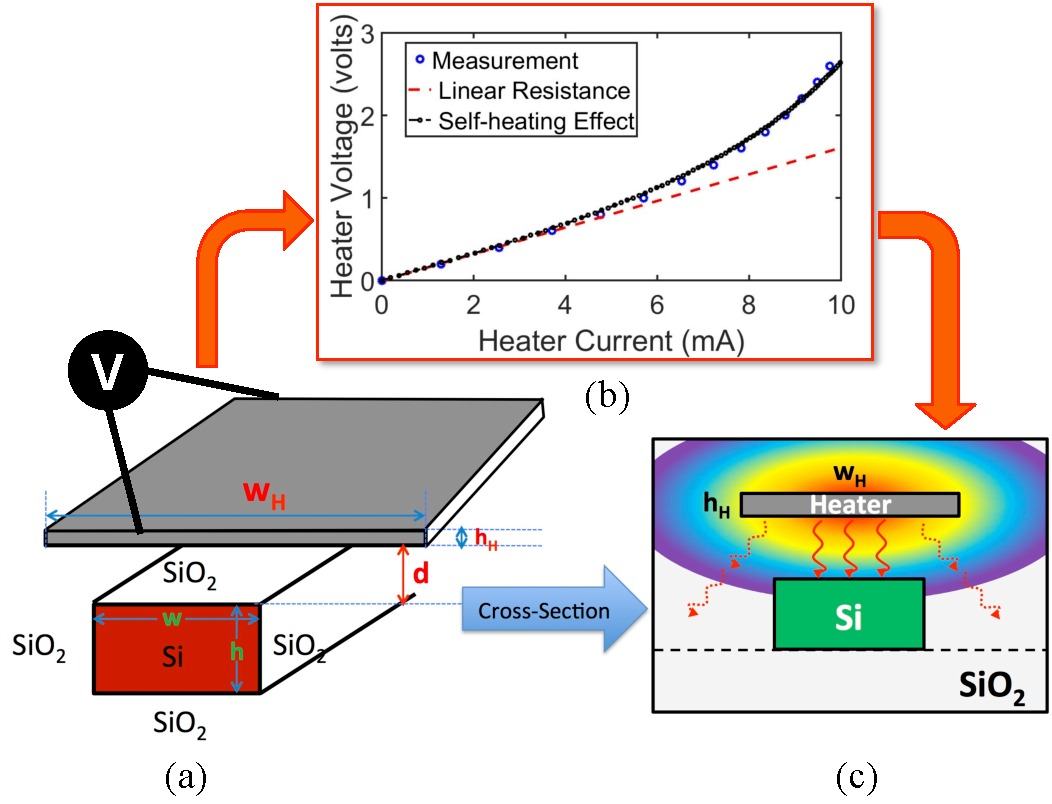
\includegraphics[width=8.5cm]{Chapter2/CH3_fig2.pdf}
\caption{(a) Structure of strip waveguide with a metallic heater situated at a distance $d$ above it. (b) V-I characteristic of the resistive heater. The nonlinear behavior is observed. (c) Schematic of heat generation at the heater and its distribution in the cladding. Dimensions are not necessarily to scale.}
\label{CH3_fig2}
\end{center}
\vspace{-0.65cm}
\end{figure}





- high capacity at low energy consumptiion

--> Phase control
--> Thermal control --> carrier injection and depletion 
--> different types of heater
--> thermal control in Mach-Zehnder vs ring 
--> response time and steady state

\section{Thermal control with pulse-width modulation}

along with a digital feedback loop for thermal control requires a large number of electrical I/O connections. Monitoring the optical operation with PWM signals has the potential to control each device with a single digital control line \cite{zecevic2015integrated, aguinaldo2014wideband}.  The main issue is to identify the frequency at which these PWM signals must be generated to obtain a stable thermal response, hence ensuring consistent optical operation. 


In the first step of our analysis we review related work (Section II) and present a preliminary analysis of the temperature sensitivity of waveguides (Section III). We then introduce an approximate analytic modeling framework for heater structures commonly used in silicon photonics platform, with an emphasis on metallic heaters. In particular, we remark that the thermal response is fundamentally governed by the heat diffusion equation. We also derive a set of expressions to describe the nonlinearity of the V-I curve of heaters, which leads us to estimates of the transient thermal response of the heater-waveguide system. We leverage this framework to analyze the thermal bandwidth of classical heater-waveguide systems (Section IV). Our analyses show that the 3dB thermal bandwidth is linearly proportional to the thermal diffusivity of the cladding material \cite{atabaki2010optimization}. To the best of our knowledge, this is the first time such a frequency model for thermal response of silicon photonic devices is proposed to characterize the trade-off between thermal bandwidth and thermo-optic efficiency. We validate our modeling framework against Finite Element Method simulations (Section V).


In the second step of our analysis we leverage our analytic framework to examine thermal rectification with a pulse width modulation (PWM) drive scheme (Section VI). In particular, we derive the relationship between the duty cycle and the required frequency of PWM excitation to obtain desired temperature conditions. These analytic conclusions are examined against experimental measurements (Section VII). Again, to the best of our knowledge, this is the first comprehensive study of PWM signaling for thermal monitoring of silicon photonic devices. 



\section{Photo-conductance effect in doped heaters}

By using the asterisk to start a new section, I keep the section from appearing in the table of contents.
If you want your sections to be numbered and to appear in the table of contents, remove the asterisk.

%This is the third chapter of the dissertation

%The following command starts your chapter. If you want different titles used in your ToC and at the top of the page throughout the chapter, you can specify those values here. Since Columbia doesn't want extra information in the headers and footers, the "Top of Page Title" value won't actually appear.
\pagestyle{plain}


\chapter[Cascaded Silicon Photonic Ring Resonators Architecture for Reconfigurable WDM Applications][Top of Page Title]{Programmable Cascaded Microring Resonators for Reconfigurable WDM Applications}

\textit{\textbf{Abstract -} In this chapter we introduce a widely used architecture of cascaded microring resonators that share a common waveguide bus. Based on the photonic design, we develop a power-aware algorithm on an FPGA platform that controls the spectral responses of the microrings to enable optical unicast, multicast and broadcast of WDM signals. The system demonstration consists of an optically and electrically packaged SiP chip with an array of eight microrings and a fast tunable C-band laser delivering programmable wavelength and spatial switching capabilities.}

\textit{We characterize the thermo-optic response of microring resonators and extract key parameters necessary for the development of the control-plane. The performance of the proposed architecture is tested with 10 Gb/s data rate and error-free operation is verified for various switching scenarios. Based on the tuning efficiency, electrical power and energy consumption is determined to reconfigure the SiP chip in the ITU grid for all possible wavelength operations and output ports combinations and show that unicast, multicast of two, three, four, five, six, seven, and broadcast functions are achieved with energy overheads of 0.02, 0.07, 0.18, 0.49, 0.76, 1.01, 1.3, and 1.55 pJ/bit, respectively.}

\textit{Utilizing the system, we further expand the control algorithm to demonstrate a programmable optical power distribution functionality. The abstraction of the physical layer allows to achieve precise power profiles profiles from the drop ports of the MRRs.}

\section{Introduction}

Today's DCs are experiencing an unprecedented increase in network traffic due in particular to the popularity of video streaming services and cloud-based computing \cite{hashem2015rise}. Server and network virtualization further exacerbate the trend \cite{wang2010impact}. This creates bottlenecks in data movement between DCs racks and processing workloads inside the rack. To address this high demand, new network architectures are proposed to provide bandwidth and resource allocation \cite{wen2016flexfly} for intra \cite{yan_FPGA_DC} and inter  \cite{kachris2012survey,bergmanoptical} racks through reconfigurable optical interconnects. These architectures, including Proteus \cite{singla2010proteus} and MORDIA \cite{farrington201310,aguinaldo2014energy}, achieve flexible networking through optical spatial switching \cite{farrington2012demonstration} or optical wavelength switching \cite{zhang2012experimental}, and augmented with optical multicasting \cite{samadi2015optical,brunina2011building}.  

In spatial switching, data carried on an optical carrier is deflected to any of the of the output ports in a configurable way. The term spatial is used to underline the fact that only the spatial routing of the light is modified. In wavelength routing, in contrast, received optical signals can be further decomposed in wavelengths, and the propagation direction of each of these wavelengths can be separately configured. Finally, in optical multicasting, incoming optical signals can simultaneously be forwarded to more than one output ports simultaneously \cite{chen2011survey}.

Most of the deployed optical switches, however, rely on discrete optical elements such as micro electro-mechanical systems (MEMS) actuated micro-mirrors arrays or Liquid crystal on silicon (LCOS) matrices \cite{robertson2014demonstration,hamza2016free,wavelength2016}. The individual cost of these elements, and sometimes their bulkiness and mechanical susceptibility, is a severe hindrance to a high utilization in large scale interconnects. To be widely deployed in datacenters as in other systems involving large data exchanges, compact, power-efficient, and above all, scalable switches are required. Silicon photonics (SiP) has emerged over the last decade as a platform for development of photonic integrated circuits (PICs) \cite{komljenovic2016heterogeneous,alloatti2015photonics}. Thanks to the utilization of already available advanced silicon based CMOS electronics foundries to fabricate and package PICs \cite{novack201330,leemeeting,bogaerts2005nanophotonic}, SiP inevitably enables significant cost reductions at scale while chip-level integration guarantees compactness. Numerous SiP integrated components have been implemented ranging from passive wavelength splitters and filters to active modulators and switches \cite{lu201616,biberman2011broadband,subbaraman2015recent}. To orchestrate these many individual SiP devices within a full network, however, a unified control plane is required \cite{calhoun2016hardware,chen2015programmable} to set the proper command signals. 

In 2011, Xu \textit{et al.} \cite{xu2011hybrid} demonstrated a SiP-based hybrid optical wavelength selective switch (WSS) platform that can potentially be utilized in data centers. The demonstrated WSS was a 1$\times$2 switch based on SiP microring resonators and showed error free performance for both OOK and DPSK optical modulation. However, a comprehensive control plane architecture to control silicon photonics and external components was not demonstrated in this work. In 2014, Calhoun \textit{et al.} \cite{calhoun2014dynamic} discussed the importance of the capability of silicon photonic switches in terms of dynamic configurability. They used 2$\times$2 broadband SiP Mach-Zehnder switch and a 1$\times$2 WDM demultiplexer based on microring resonators. Quite interestingly, this work focused on a unified control plane to orchestrate the photonic devices side-by-side. However, the demonstrated system still lacked to portray a picture of how the control plane would evolve if the system scales up and did not support routing of complex patterns such as multicast. 

In this chapter, we describe a system based on a common array of cascaded microring resonator (MRR) in the form of a packaged SiP chip, connected to an external Y-branch fast tunable laser \cite{browning2013optical}. The control over the SiP chip and the laser is developed on an FPGA platfrom and abstracted into a single programmable command. The control algorithm is optimized to achieve minimum energy consumption due to thermal control \cite{biberman2008thermally} of the SiP chip for all possible wavelength and spatial switching scenarios. To the best of our knowledge, it is the first time that a control plane capable of performing optical multicast in SiP platform utilizing a single wavelength source is demonstrated. In the experimental demonstration we examine the transmission quality of incoming 10Gb/s OOK signals in terms of eye-diagram and BER from unicast to broadcast of eight at various operational wavelengths. 

In the last section of the chapter, we further expand the control algorithm to demonstrate a programmable optical power distribution using the same system architecture. First, a motivation for such functionality is presented and then experimental results of precise power profiles are shown within several percent error margin from the programs input.

\section{System architecture and functionality}


Figure \ref{fig1} shows a block diagram of the proposed system architecture. The main components are a fast tunable laser (TL), a SiP chip, two field programmable gate arrays (FPGAs) and a computer that provides an interface to the user. Depending on the desired configuration, the computer sends operation messages to the two FPGAs via a serial data transfer interface. One FPGA translates the messages into command signals for the TL to adjust its output optical power and the wavelength of operation over the C-band. The other FPGA controls the spectral responses of an array of eight cascaded MRRs. As shown in Fig. \ref{fig1}, an external modulator is used to encode data onto the laser output. Through software abstraction of the physical layer, the system is capable routing incoming optical data to any of the eight output ports, as well as splitting the incoming data (multicasting) to a number of output ports by precise and predetermined control voltages on each MRR. 

\begin{figure}[b]
\begin{center}
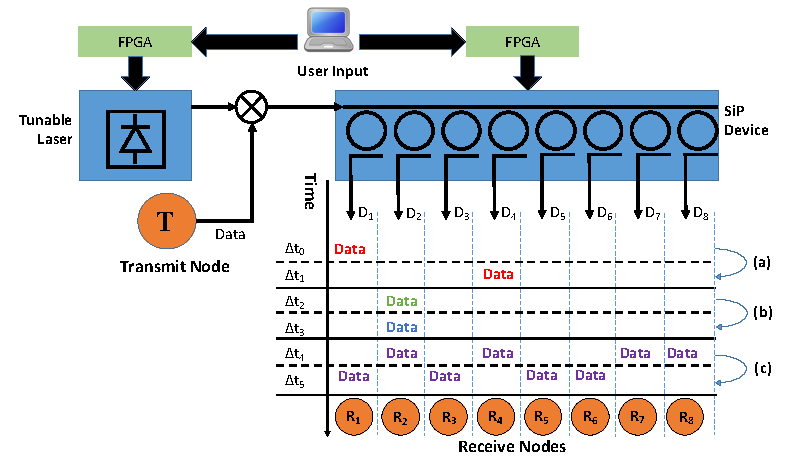
\includegraphics[width=13cm]{Chapter3/fig1.pdf}
\caption{Block diagram of the system including a tunable laser, SiP device, and two control FPGAs. The data modulates the laser's wavelength and is transmitted through the SiP device. The central control computer can reconfigure the tunable laser and the SiP device to switch the data to any number of the eight ports (a), wavelength routing (b), and multicasting (c).}
\label{fig1}
\end{center}
\vspace{-0.9cm}
\end{figure}

The time-slot diagram in Fig. \ref{fig1} illustrates three possible operation of the system. In this example, the different colors of the \textit{Data} in the figure correspond to different wavelengths of the TL. During slot $\Delta t_0$ the data stream is routed to output R1. In between $\Delta t_0$ and $\Delta t_1$ slots the data stream is switched to output R4  (Fig. \ref{fig1}(a)) without changing the operating wavelength (red color). In the second case, shown in Fig. \ref{fig1} (b), wavelength routing is performed. During time slot $\Delta t_2$ the data is transmitted to output R2 on a carrying wavelength $\lambda_1$ (green color) while in slot $\Delta t_3$ the output port stays the same but the wavelength changes to $\lambda_2$ (blue color).  Finally, a multicast (one to many) operation is shown in Fig. \ref{fig1}(c). During slot  $\Delta t_4$, an incoming data stream modulated on a user's chosen wavelength (purple color) is split among four output ports: R2, R4, R7, and R8.  In the following time slot  $\Delta t_5$, the recipients of the multicast operation are modified to R1, R3, R5, and R6. The transition time between the time slots is determined by the reconfiguration time of either the TL ($\sim$ 10 ns \cite{browning2013optical}) or the SiP device ($\sim$ 20 $\mu$s) from the moment the FPGAs apply the command signals.

The operation of the system is not limited to the particular sequential illustration presented in Fig. \ref{fig1}.  Because the TL can operate at 40 distinct wavelength channels in the C-band ITU grid, and the SiP device can perform unicast (one to one), multicast (one to many), and broadcast (one to all) operations, numerous deterministic combinations are possible without any constraints. 

\section{SiP control plane}

\begin{figure}[t]
\begin{center}
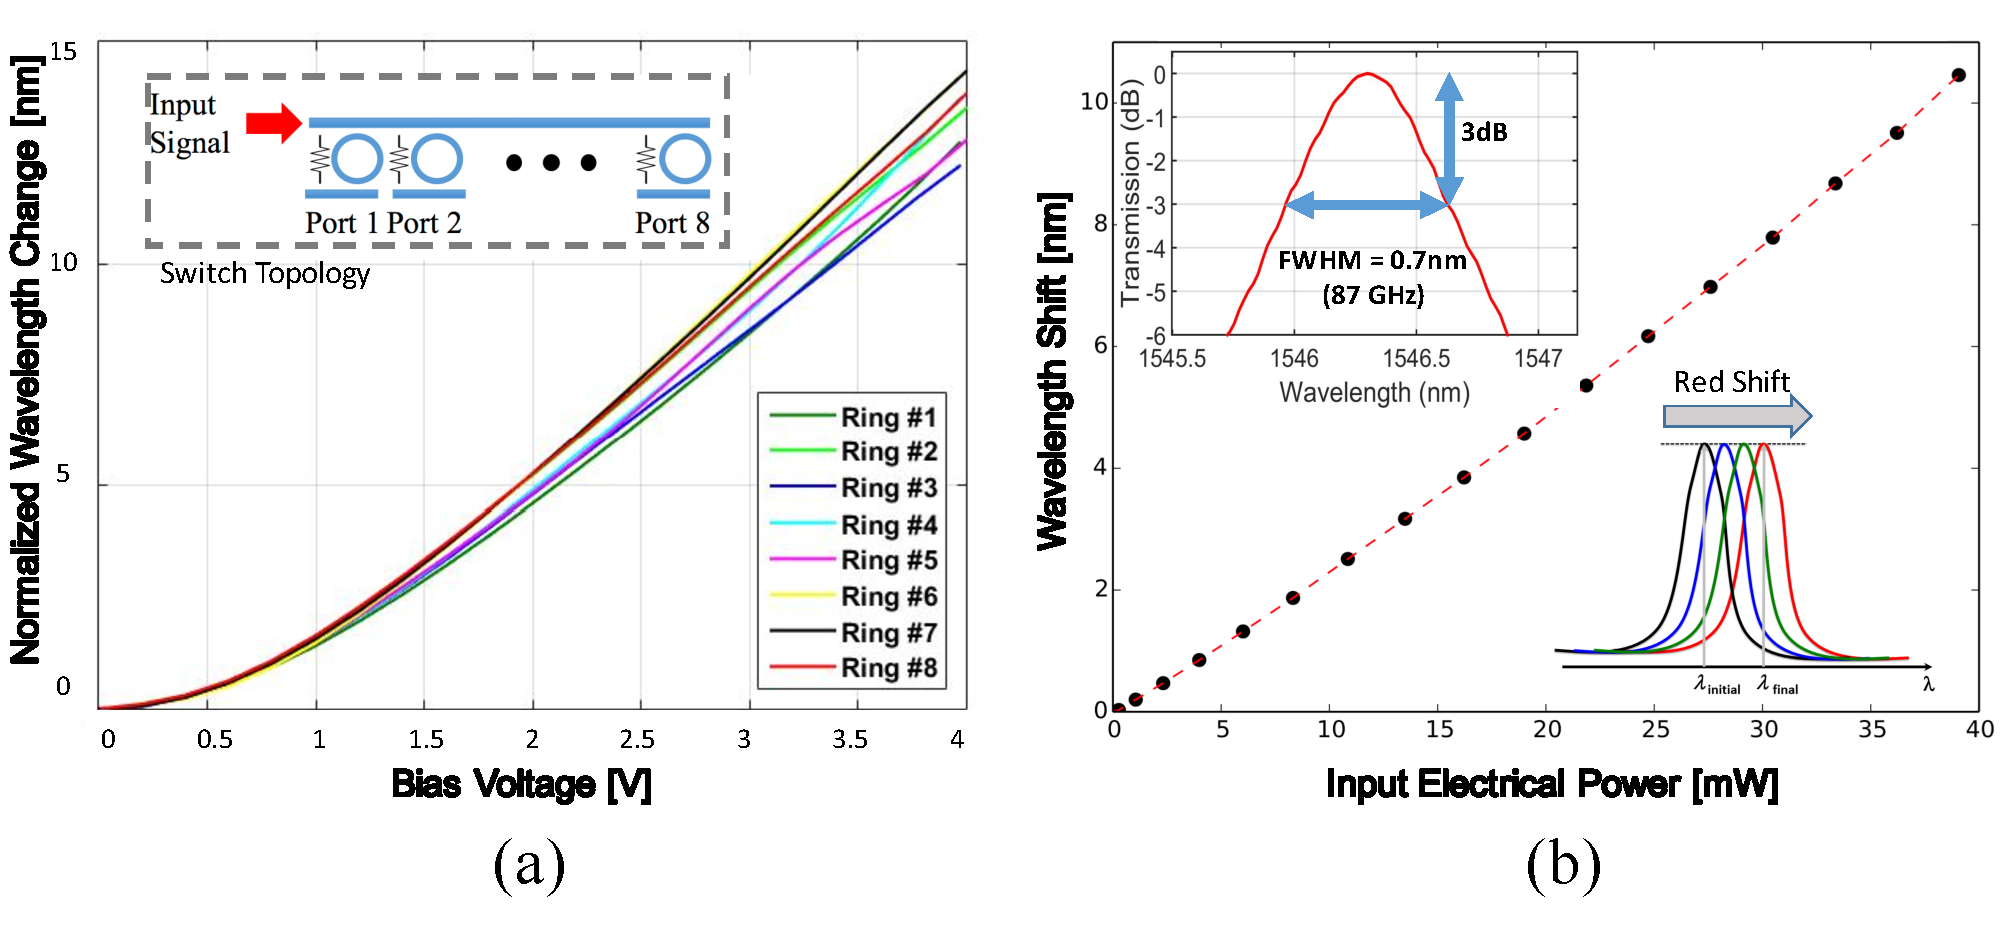
\includegraphics[width=13cm]{Chapter3/fig2.pdf}
\caption{(a) Measured thermo-optic response of the heater-ring system of the eight rings. Inset illustrates a schematic of the SiP device where each MRR has its own individual resistive heating element. (b) Averaged shift of resonance as a function of dissipated power in eight rings. Bottom inset illustrates a red shift and the top inset shows the measured 3dB bandwidth of each drop port.}
\label{fig2}
\end{center}
\vspace{-0.9cm}
\end{figure}

%%%%%%%%%%%%%%%%%%%%%%%%%%%%%%%%%%%%
%\textbf{Through integration of micro-heater on top of each MRR, the large thermo-optic coefficient of silicon \cite{komma2012thermo} can be leveraged to precisely control the rings' spectral responses. Although precise, thermal control is limited to the micro-second \cite{atabaki2010optimization} regime in our demonstration. Faster control could be achieved by injecting or depleting charge carriers into/from the silicon waveguides to control the resonance \cite{wu2015compact}. The proposed architecture relies on the fast tunable laser with nano-second timescale reconfiguration \cite{browning2013optical} in order to bypass the slower thermal response of the SiP MRRs. Nevertheless, the reconfiguration of the SiP device is required whenever multicast functionalities and broadcast are demanded. }
 
To obtain reliable reconfigurability of the packaged SiP device, a characterization of the dynamic behavior of each MRR must be performed. The MRRs are designed with varying radii around 7$\mu$m enabling different wavelengths of operation when no bias is applied. The inset of Fig. \ref{fig2}(a) shows a schematic of the SiP chip where each MRR has an electrical interface to a resistive heating element fabricated on top \cite{atabaki2010optimization}. Due to the high thermo-optic coefficient of silicon \cite{komma2012thermo}, an increase in the supplied voltage to the heater increases the local temperature of the ring and causes a change in the effective index of the optical mode allowing the resonance of the rings to shift to higher wavelengths (red shift). To achieve accurate and error-free switching operations, the thermo-optic response (shift of resonance vs. applied voltage) of each individual ring is measured and stored in the control plane. To that end, the optical signal is coupled to and from the chip through an aligned and glued fiber-array directly on top of the embedded grating coupler structures. Fig. \ref{fig2}(a) shows normalized responses as a function of increased bias voltage. Second order polynomial functions have been fitted to the measured results allowing a continuous and accurate relationship between the supplied bias voltage and the frequency response. These functions together with MRRs' Lorentzian resonant response \cite{bahadori2016comprehensive} (e.g. 3 dB bandwidth of 87 GHz shown in the inset Fig. \ref{fig2}(b)) and zero bias resonances are used in the control algorithm to perform any type of switching operation.
 
\begin{figure}[b]
\begin{center}
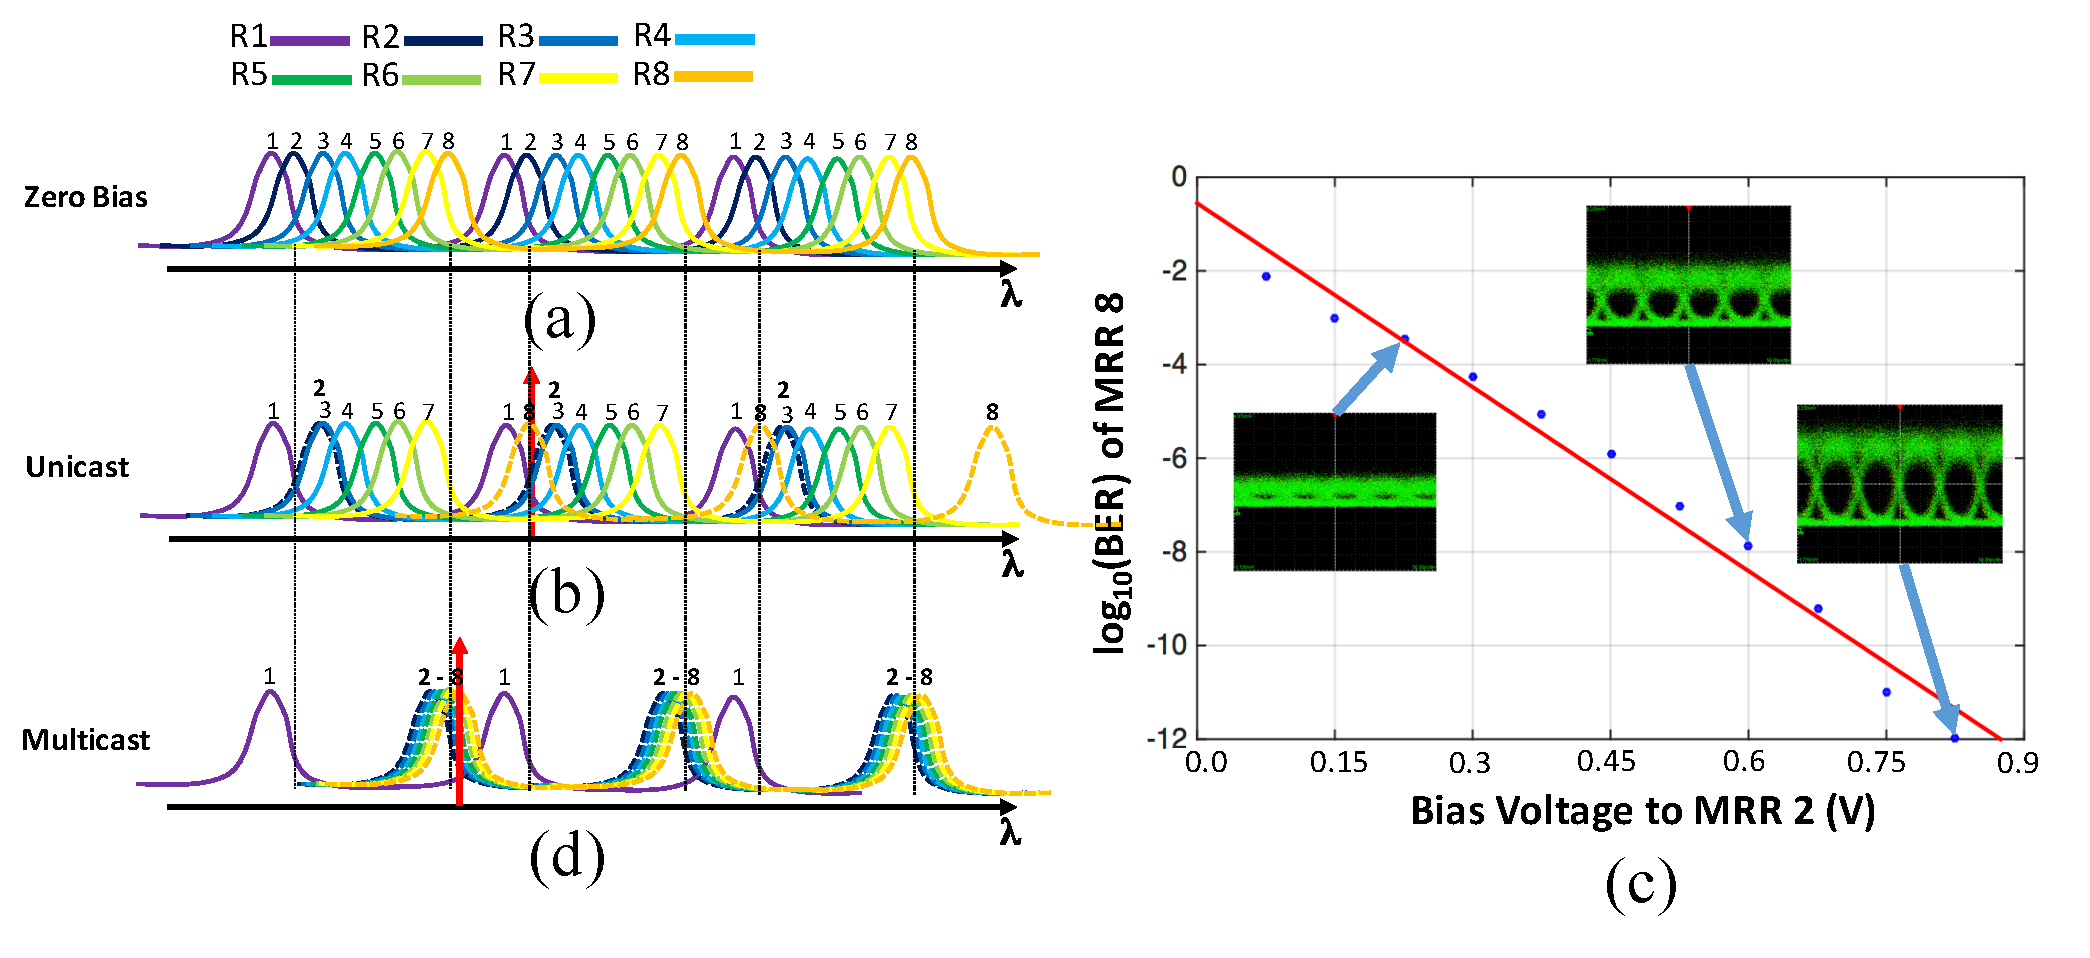
\includegraphics[width=13cm]{Chapter3/fig3.pdf}
\caption{(a) Illustration of the spectral response of the chip with zero bias. (b) Illustration of the spectral response of the chip in unicast operation. (c) Demonstration of a detuning procedure where 10Gbps data is modulated on wavelength  1543.09 and both MRR 2 and 8 are tuned to the same resonances. (d) Illustration of the spectral response of the chip in multicast operation.}
\label{fig3}
\end{center}
\vspace{-0.9cm}
\end{figure}

In addition, the electrical power dissipated by the heaters as a function of the resonance shift is shown in Fig. \ref{fig2}(b). A slope of 0.266 nm/mW defines the tuning efficiency. We utilize this parameter to estimate the range of the required power overhead (minimum and maximum) to perform all possible switching cases (unicast, multicast, and broadcast).

\subsection{Unicast, multicast and broadcast functionalists}

In order to achieve different data routing operations, the TL, via its control FPGA, is set to the desired transmission wavelength, while the SiP chip's control FPGA is instructed to supply bias voltages necessary to shuffle spectral responses based on the chosen data routing operation. Figure \ref{fig3}(a) illustrates the responses of the MRRs in our chip when no bias voltage is applied. By design, the responses of the rings are separated by 1.27 nm ($\sim$ 160 GHz) with an FSR of 13 nm and 3 dB bandwidth of 0.7 nm.

-->>I AM HERE<<--

Figure \ref{fig3}(b) shows a unicast operation where the input data on the wavelength denoted by a red vertical arrow is routed to output port 8 (dashed black curve). To obtain this mode of operation, i) the resonance of ring R2 must be detuned to prevent dropping at port 2 because R2 has the precedence over R8 in the MRR array, and ii) the resonance of ring R8 must be tuned to the red wavelength. The amount of detuning required for ring R2 to achieve error free operation is obtained experimentally and demonstrated in Fig. \ref{fig3}(c). As the bias voltage over R2 is increased gradually, its resonance is shifted to allow the signal to propagate to R8. The bit-error-rate (BER) and the eye-diagrams are captured at output port of R8 to verify the amount of detuning necessary in order to reach the error free transmission (BER = 10$^{-12}$) with negligible crosstalk effects \cite{bahadori2016crosstalk}. At a bias of 0.85 V the signal is fully routed to the output port 8. We estimated that this amount of detuning is about 1.08 nm which corresponds to a channel suppression of 10 dB between the desired output port (R8) and the detuned MRR (R2). This amount of detuning is chosen for power efficiency; any further detuning will cost more energy-per-bit while introducing negligible improvement on the BER of the routed 10 Gbps OOK signal. 

Figure \ref{fig3}(d) illustrates a one-to-seven multicasting operation. This operation is possible by aligning the Lorentzian response of each MRR so that the power of the optical signal is divided equally among the desired output ports; i.e. tuning the rings to the appropriate resonances, starting from the last MRR participating in the multicast operation. The last MRR, R8 in this example, is tuned so that its resonance aligns exactly with the TL wavelength, allowing maximal transmission over its drop path. R7 is then tuned to its 3dB bandwidth point, allowing a drop of 50\% of the optical power. Continuing with this approach R6, R5, R4, R3 and R2 are tuned to the following drop power ratios: 33.33\%, 25\%, 20\%, 16.67\% and 14.28\%, respectively, i.e. following a harmonic series (1, 1/2, 1/3, 1/4 $\dots$). When the process is complete, each of these seven rings will equally drop 14.28\% of input optical power coupled into the SiP chip. Realizing multicast exhibits the fine tuning levels our system is capable of, and demonstrates the potential of SiP for error-free multicast operation of one stream of data over a single wavelength.


%****************************
\subsection{Software implementation }

Once the SiP device is fully characterized, collected measurement data can be exploited by an algorithm to find the ideal device settings corresponding to a specific configuration.

\begin{figure}[b!]
\begin{center}
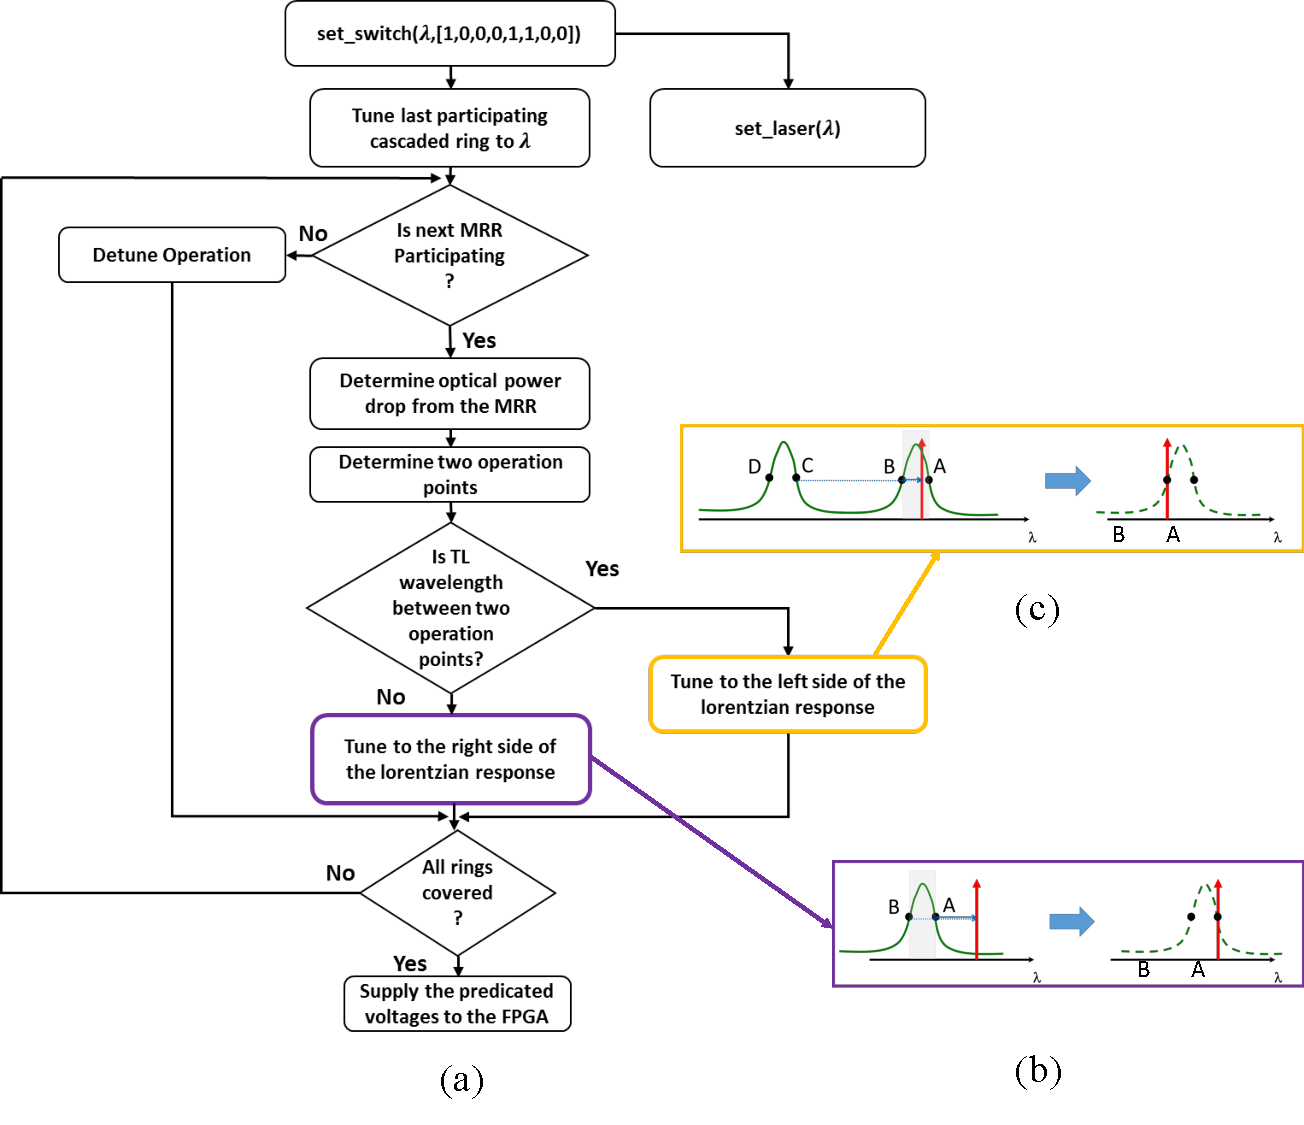
\includegraphics[width=13cm]{Chapter3/fig4.pdf}
\caption{(a) The flowchart of the control algorithm to achieve optimal tuning. (b) If the laser wavelength is located outside the two possible tuning points (A and B), point A is selected. (c) If the laser falls between the A and B tuning points, point A is not accessible. Therefore, point B is targeted as it requires less tuning power than point C or D.}
\label{fig4}
\end{center}
\vspace{-0.9cm}
\end{figure}

The flowchart in Fig. \ref{fig4}(a) describes our algorithm to configure the SiP chip for all possible switching cases. We implemented the algorithm in a host computer in Python and post calculation commands are sent to the two FPGAs that control the TL and the SiP device, respectively.



The algorithm takes two arguments. The first is channel number, which determines the wavelength of operation for TL, and the second argument is a binary array indicating where to route the signal. For example, \textit{set\_switch(ch1,[0,1,0,0,0,0,0,0])} will route the input data on wavelength $\lambda_1$  to output port R2 and \textit{set\_switch(ch2,[0,1,0,1,1,1,1,1])} will perform a multicast of the input data on wavelength $\lambda_2$  to output ports R2, R4, R5, R6, R7 and R8. The resonance of the MRR corresponding to the last selected port is always tuned exactly to the selected channel in order to provide a 100\% drop of power. The resonance of the next selected port will be set to achieve 50\% drop and so forth. For the unselected ports, our software executes an adaptive detune operation in which it determines if the MRR needs to be shifted from the 10 dB region or can be left untouched. After the main loop is completed, the amount of the required wavelength shifts for the MRR array are converted to corresponding bias voltages and sent to the control FPGA of the SiP device.

Due to the symmetrical spectra of the MRRs it is possible to drop the required amount of optical power from either side of the Lorentzian response. To optimize the tuning power consumption of the MRR array the software automatically selects the closest tuning option. Fig. \ref{fig4}(b) shows the case where the laser (red arrow) is outside of the two possible tuning points (markers A and B). After the execution of the algorithm, the nearest point (A) is aligned with the laser. Figure \ref{fig4}(c) depicts the case where the laser wavelength falls in between the two possible operation points (markers A and B). In this example, the MRR will be shifted to the left, to align with point B. Note that in this case the point on the right side of the laser (marker A) is not accessible due to the red-shift nature of thermal tuning. Using the two sides of the Lorentzian response, in this particular case, avoids reaching point C, which requires a large heater power. 


%%%%%%%%%%%%%%%%%%%%%%%%%%%%%%%%%%%%%%%%%%%%%%%%%%%%%%%%

\section{Experimental demonstration and evaluation}

The schematic of the experimental setup is shown in Fig. \ref{fig5}. A tunable Y-branch laser \cite{browning2013optical} (Fig. \ref{fig5}(a)) mounted on an FPGA board was used to output light at various frequencies across the ITU 100 GHz C-band grid. The packaged SiP device along with its control plane is shown in Fig. \ref{fig5}(b). The control plane is based on an Stratix III EP3SL150 FPGA (separate from the laser) capable of hosting and controlling eight parallel digital-to-analog converters (65 MHz DAC) with 14 bits of resolution. An image of the DACs mounted on top of the FPGA is marked by (1) in Fig. \ref{fig5}(b). The output voltage from the DACs (0--1 V) is amplified by 5 in the gain stage (marked as (2)) to achieve a full FSR swing for each MRR. The amplified control signals are connected to a break-out printed-circuit-board (PCB) (marked as (3)) which hosts the SiP chip. After fabrication, the chip was attached to, and wire-bonded on, a standard electrical IC package (marked as (4)). The silicon photonic chip used in this work is not equipped with any temperature sensors, so no active temperature stabilization procedure is included in the design of the chip. However, the chip is sitting on a heat sink in the IC package that passively regulates its temperature to the ambient temperature level. An array of optical fibers is glued to the packaged chip on top of grating couplers (marked as (5)). 

\begin{figure}[t!]
\begin{center}
\includegraphics[width=13cm]{Chapter3/fig5.pdf}
\caption{(a) An image of a fast, C-band tunable laser. (b) Schematic of the experimental setup. Pulse Pattern Generator (PPG), Erbium Doped Fiber Amplifier (EDFA), Mach Zehnder Modulator (MZM), Bit Error Rate Detector (BERT), Avalanche Photodiode (APD), Trans-Impedance Amplifier (TIA), Variable Optical Attenuator (VOA), Polarization Controller (PC), Optical Spectrum Analyzer (OSA), Optical Bandpass Filter (OBPF). (c) Packaged SiP device with its control plane: (1) four dual DAC cards on an FPGA development board, (2) electrical Gain stage (3) breakout PCB (4) packaged and wire-bonded SiP (5) An array of ten fibers glued on the SiP chip. }
\label{fig5}
\end{center}
\vspace{-0.9cm}
\end{figure}

To test various switching scenarios, a PPG was used to output a 10 Gbps PRBS (2$^{31}$-1) signal, which was then electrically amplified before being modulated onto the optical carrier using a Mach-Zehnder modulator. The optical signal was then sent to the SiP device, configured through the software control plane, to route the signal to the desired output port(s). Because the SiP chip exhibits coupling loss of $\sim$ 25 dB due to its packaging, in our experiment an EDFA was required to amplify the received signal. Using a 1:3 divider, the optical signal was directed to an OSA, an oscilloscope to observe the received eye diagram and an APD. The power falling on the APD was kept at a constant level of -8 dBm to avoid saturation. The output of the photo-receiver was sent to the bit error rate tester (BERT) for BER measurement. The BERT and oscilloscope were both triggered with the same clock signal from the PPG.


%****************************
\subsection{Unicast}

Figure \ref{fig6} maps all possible unicast combinations based on wavelength and spatial routing capabilities of the system. The spatial ports are denoted in the vertical axis where MRR 1 corresponds to the first output port in the cascaded topology. The horizontal bars illustrate the tuning range of each MRR with a zero bias resonance at the grey vertical lines. The thin vertical dashed lines separated by 100GHz correspond to the all possible optical channels of the TL. The thicker dashed lines and the eye-diagrams to their right indicate the TL channels and the drop port combinations which were used in our experiment. 

A 10Gbps optical signal was injected into the input port of the chip and various wavelength routing and spatial switching configurations were tested in order to confirm error-free operation (in these cases all measured BER $\leq$ 10$^{-12}$) operation. The control plane was first set to test spatial switching, where data carried on a specific wavelength was switched from one drop port to another. The TL laser was set to channel 22 (1541.70 nm) and the signal quality (Eye diagram and BER) was monitored over four different switching cases for drop ports of MRRs 1, 2, 3 and 4. Similarly, The TL was set to channel 13 (1551.28 nm) and the control plane configured the SiP for four different cases to route the data to the output ports 5, 6, 7, and 8. 

Next, wavelength routing was tested where the data is routed through a specific port, each time with a different wavelength. The eye-diagram and BER were captured at port R1 while the control plane reconfigured the transmitted wavelengths to 1533.81 nm, 1537.75 nm, 1541.70 nm, and 1549.67 nm. In a similar measurement, the signal quality was measured at port R8 with the following wavelengths: 1529.12 nm, 1543.29 nm, 1551.28 nm, and 1560.97 nm.

The results of this part of our experiment demonstrate the capability of the SiP-based system for error-free optical unicast operation.


%****************************
\subsection{Multicast and broadcast}

\begin{figure}[t!]
\begin{center}
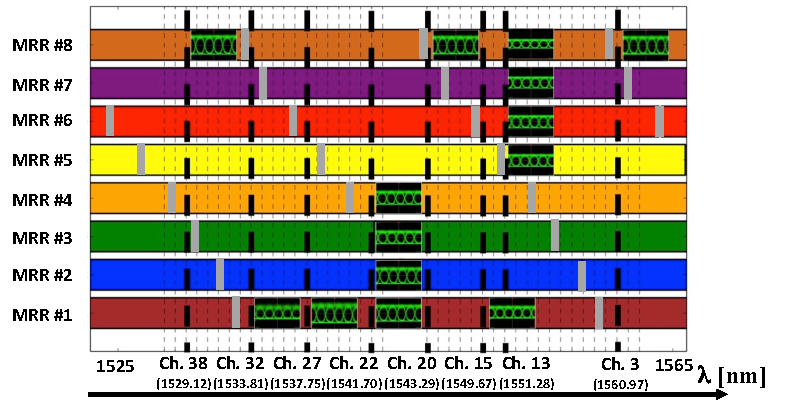
\includegraphics[width=13cm]{Chapter3/fig6.pdf}
\caption{Tuning ranges of eight cascaded MRRs in the C-band. The eye-diagram plots are captured from experimentally tested error-free unicast operation at various combinations of wavelength and output ports. Color strips are used to differentiate the outputs. }
\label{fig6}
\end{center}
\vspace{-0.9cm}
\end{figure}

Figure \ref{fig7} shows experimental measurements for multicast and broadcast operations, and the best and worst power consumptions for each operation. All the results were set to perform at channel 17 of the laser (1548.11 nm). First, the control plane was set to route the data to R2. Then the SiP device was reconfigured to multicast the data to ports R2 and R7. The BER and the eye-diagrams were captured at the two output ports separately to verify error-free operation. This process continued to higher multicast port counts until it covered all the eight ports (broadcast). The tested multicast cases are marked by eye-diagram results in each row of Fig. \ref{fig7}. 

\begin{figure}[t!]
\begin{center}
\includegraphics[width=13cm]{Chapter3/fig7.pdf}
\caption{Experimental results of 8 different cases including Unicast, Multicast and Broadcast operated at 1548.11nm are shown in first 8 columns. The last column shows the estimation of best and worst case power consumption for all possible configurations. }
\label{fig7}
\end{center}
\vspace{-0.9cm}
\end{figure}

The column on the right side of Fig. \ref{fig7} shows power overhead analysis due to the reconfiguration (thermal tuning) of the SiP device. All possible combinations of TL wavelengths and SiP output ports were swept in order to determine the best and the worst case of power consumption. The results were achieved by estimating the amount of wavelength shift (in nm) necessary for each MRR, converting it to ohmic power (in mW), and summing them up to get the overall mW consumption. With a data rate of 10 Gbps, the static ohmic power of each participating MRR was also converted to energy per output-bit (pJ/bit) overhead. Finally, the total pJ/bit was obtained by adding all the individual pJ/bit values.

For example, for multicast using 3 ports, the best power consumption is calculated to be 5.37 mW for the \textit{(ch32,[1,1,0,0,0,0,0,1])} combination with an energy overhead of 0.18 pJ/bit. While the worst combination is \textit{(ch19,[1,0,0,0,0,0,1,1])} resulting in an ohmic power of 120.97 mW and an energy overhead of 3.94 pJ/sent-bit (1.31 pJ/received-bit).

\section{Programmable optical power distribution}

Building on the multicasting algorithm, we expand the control plane over the SiP cascaded MRRs to perform programmable optical power distribution. This capability can pave the way for future optical network requirements that focus on higher utilization and reduced energy consumption. 

Since the quality of transmission (bit error ratio, BER) in a digital optical links is directly related to the optical signal-to-noise ratio, pumping more optical power into a communication link will result in a better reception of the data as long as the optical power is kept below the nonlinearity threshold of the transmission medium \cite{bahadori2015nonlinear}. Additionally, the distribution of optical power can be further optimized for bandwidth and/or distance requirements of each point-to-point link \cite{ramaswami2009optical}. Optical power distribution has also the potential to reduce energy consumption in optical networks with a centralized optical source. A single high-power laser is known to achieve more than 40\% of efficiency \cite{heck2014energy} and can be utilized as an external central power source in conjunction with a dynamic power allocation routines \cite{posca2018powering}. 

To execute the programmable optical power distribution we again utilize the parameters necessary to fit the Lorentzian function describing the spetrcal response of each MRR: resonance wavelength and 3dB bandwidth as shown in Fig. \ref{fig2}. Together with the dynamic thermo-optic responses we obtain the optical drop power as function of the applied bias voltage (DR(V)). This functions are saved in the FPGA as a look-up table.

The power distribution functionality is abstracted into a single command called \textit{set\_power}($\lambda$, power, [$\alpha_1$,$\alpha_2$,$\alpha_3$,$\alpha_4$,$\alpha_5$,$\alpha_6$,$\alpha_7$,$\alpha_8$]) 
set by the user in the processor core of the Altera FPGA (nios-ii). The input entries $\lambda$ and power control the TL \cite{browning2013optical} to the desired wavelength and power in dBm units, and $\alpha_1$ to $\alpha_8$  ($\sum_{i=1}^{8}\alpha_i \leq 1$)  set the desired drop ratios from output ports 1 to 8. Due the cascaded design of the SiP chip, the user input ratios are converted to power drops based on the following relationship:
\begin{equation}\label{CH4_eq2}
DR_1 = \alpha_1, DR_i = \frac{\alpha_i}{1-\sum_{1}^{j-1}\alpha_j}
\end{equation}
As an example, for equal power distribution through the first four ports ($\alpha_1=\alpha_2=\alpha_3=\alpha_4=25 \%$) the actual programmed drop levels are set to $DR_1= 25\%$ , $DR_2= 33.3\%$, $DR_3= 50\%$, $DR_3= 100\%$ based on Eq. \ref{CH4_eq2}. The calculated drop ratios of the participating ports are translated to bias voltages, and if one of the non-participating ports’ spectral response lines up with the wavelength of operation, it is automatically de-tuned from its zero-bias operation (as shown in Fig. \ref{fig3}(b)). The optical coupling variation between the ports and the fibers is calibrated and taken into account to further increase the accuracy of the algorithm. 

\begin{figure}[t!]
\begin{center}
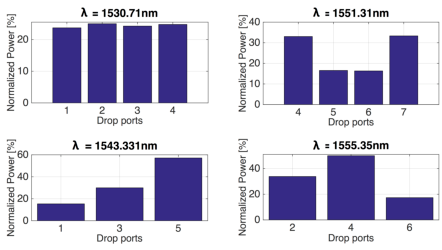
\includegraphics[width=13cm]{Chapter3/CH_3_power_dis.pdf}
\caption{Demonstration of dynamic power distribution through drop-ports of cascaded microring resonators (a) Equalized power distribution for four rings. (b) Power down and up for four rings. (c) 3dB step up for three rings. (d) Power up and down for three rings. Note that the wavelength of operation is different for each case and is set by the user.}
\label{fig8}
\end{center}
\vspace{-0.9cm}
\end{figure}

Figure \ref{fig8} summarizes the experimental results of four distinct distribution profiles at different operating wavelengths and 12dBm of laser power. Fig. \ref{fig8}(a) shows the results for equalized power profile [1/4,1/4,1/4,1/4,0,0,0] among ports 1, 2, 3 and 4 at 1530.7nm, and Fig. \ref{fig8}(b) shows [0,0,0,1/3,1/6,  1/6,1/3] profile at 1551.31nm. Fig. \ref{fig8}(c) corresponds to a ramp-up profile set to [1/7,0,2/7,0,4/7,0,0] at 1543.331nm and Fig. \ref{fig8}(d) corresponds to a mixed profile of [0,1/3,0,1/2,0,1/6,0] at 1555.35nm. The corresponding applied bias voltage array for each case are [0.97, 0.80, 1.77, 2.35,0,0,0] V, [0,0,0.48, 0.80, 1.15, 1.70, 2.3] V, [1.04,2.00,1.65,0,2.94,0,0] V and [1.04,0.90,0,2.06,0,3.09, 0] V respectively. For cases 3(b)-(d), it can be seen that bias voltages are applied to more MRRs than participating ports in the power profile. The additional MRRs are the ones that need to be de-tuned from their zero-bias operation. These results show the capability of the system to generate wavelength selective power profiles within several percent error margin from the programmed input. 









%%%%%%%%%%%%%%%%%%%%%%%%%%%%%%%%%%%%%%%%%%%%%%%%%%%%%%%%
\section{Conclusion}

For the first time, we demonstrate a fully integrated software control plane in order to realize optical unicast, multicast and broadcast in conjunction with wavelength selectivity on a silicon photonic chip.  We show that any switching configuration set by the user input could be precisely determined in an energy efficient way by our control plane. This level of abstraction of the physical layer paves the way for directly integrating SiP-based devices into a higher-level control plane under a software defined networking (SDN) paradigm. SDN and all optical routing are key requirements for next generation reconfigurable optical networks/interconnects.

Based on the static spectral response and thermo-optic behavior or silicon-based microring resonators, a control plane was developed to dynamically distribute the optical power to the drop ports of an array of seven add-drop ring resonators. We demonstrated, experimentally, various power profiles including uniform, ramp up, and mixed based on the predicted heater voltages in the control plane. 
%This is the second chapter of the dissertation

%The following command starts your chapter. If you want different titles used in your ToC and at the top of the page throughout the chapter, you can specify those values here. Since Columbia doesn't want extra information in the headers and footers, the "Top of Page Title" value won't actually appear.
\pagestyle{plain}

\chapter[Closed-loop solutions for silicon photonic ring resonators][Top of Page Title]{Closed-loop solutions for silicon photonic ring resonators}

This high thermo-optic susceptibility, on one hand, can be an opportunity as it allows for effective manipulation of the light in thermo-optic modulators \cite{nedeljkovic2014mid,gautam2012single,wang2003soi} and optical switches \cite{suzuki2017broadband,li2016silicon,liu2016two}, for example. On the other hand, for very narrow-band optical devices such as ring resonator filters, thermal susceptibility is detrimental, and  requires  accurate monitoring and control of the temperature to obtain desired behavior and performance \cite{gazmanautomated,zortman2013bit,mahendra2017multiwavelength,padmaraju2014resolving,padmaraju2012thermal}. For example, the resonant frequency of a silicon ring resonator is shifted by $\sim$9 Ghz ($\sim$0.07 nm) for each degree Kelvin change in the temperature of the waveguide \cite{masood2013comparison,pintus2016optimization}. A single degree of temperature variation is therefore sufficient to create significant spectral distortion  of on-off keying (OOK) signals for dense wavelength-division multiplexing (DWDM) systems that employ add-drop ring filters at the receiver \cite{bahadori2016crosstalk,bahadori2016energy,sun2015single}. 

Different mechanisms of thermal control and compensation have been proposed to improve tolerance of narrow bandwidth devices to ambient temperature variations. The use of polymer cladding that counteracts the thermo-optic effect of silicon has been proposed \cite{guha2013athermal}; however, this approach requires a specific width of the waveguide ($\sim$306 nm \cite{padmaraju2014resolving}) and some post fabrication processes that are not CMOS compatible. Polymers have also been used in the design of low-power thermo-optic switches \cite{niu2017optimized}. The most popular solution leverages active thermal control and consists of sending an electrical current through external but closely integrated metallic \cite{atabaki2010optimization} or doped-silicon based micro-heaters to induce ohmic heating \cite{pintus2016optimization}. Fabrication constraints require metallic heaters to be located above the waveguide and doped-silicon heaters to be located next to the waveguide. In both cases, the generated heat diffuses mainly through the silica (SiO$_2$) cladding layer to reach the silicon waveguide \cite{masood2013comparison,niu2017optimized}. Solutions where the waveguide itself is turned into a heater by tapering it to a wider width and doping it locally have also been proposed in \cite{watts2009adiabatic, derose2011low}, and \cite{watts2013adiabatic}. An approach consisting of a PN-doped waveguide driven with a reversed voltage to its breakdown to produce Ohmic heat right inside it has also been proposed by Li \textit{et al}. \cite{li2014fast}. Heat diffusion by means of external heaters, however, permits a separation between the design of the waveguide (choice of optical mode and polarization) and the design of the heating element.


\section{Introduction}

By using the asterisk to start a new section, I keep the section from appearing in the table of contents.
If you want your sections to be numbered and to appear in the table of contents, remove the asterisk.
\section{Sensitivities in Micro Ring Resonators}
\section{Micro-ring resonators sensitivity issues: fabrication variations, thermal sensitivity and self-heating}

By using the asterisk to start a new section, I keep the section from appearing in the table of contents.
If you want your sections to be numbered and to appear in the table of contents, remove the asterisk.


%This is the first chapter of the dissertation

%The following command starts your chapter. If you want different titles used in your ToC and at the top of the page throughout the chapter, you can specify those values here. Since Columbia doesn't want extra information in the headers and footers, the "Top of Page Title" value won't actually appear.
\pagestyle{plain}

\chapter[Tapless and design agnostic Silicon Photonic spatial switches][Top of Page Title]{Tapless and design agnostic calibration of Silicon Photonic spatial switches}

\textit{\textbf{Abstract - }We leverage the photo-conductance (PC) effect in the doped phase-shifter heaters for both controlling and calibrating the Mach-Zehnder interferometer (MZI) switch elements. Both the steady-state and the transient response are experimentally characterized and compact models for the PC current are developed. Utilizing the PC effect, a topology agnostic algorithm is then outlined. The calibration procedure is experimentally verified against calibration with external photo-detectors using a non-blocking 4$\times$4 Benes switch consisting of six 2$\times$2 MZIs. It is shown that our PC-based approach agrees with the PD-based procedure within less than 2.5\% of difference between the obtained calibrated values. Based on the calibrated PC values, all possible routing configurations are measured for extinction ratio (9.92--21.51dB), insertion loss (0.88--4.59dB), and exhibiting performances far below the 7\% FEC limit (bit error rate of $3.8\times 10^{-3}$) using 25 Gbps 4-level pulse-amplitude-modulation signals (PAM4).}
 sb

\section{Introduction}

The continuous increase in data-center traffic is pushing the bandwidth limits of conventional network interconnects\cite{Cisco_whitePaper}. Low power consumption, small footprint, and CMOS integration compatibility are all characteristics of the Silicon Photonic (SiP) broadband switches that promote them as promising building blocks for realizing new reconfigurable inter- and intra-datacenter optical network architectures\cite{Cheng_DC}. Through steering and readjusting the end-to-end nodes interconnectivity\cite{Shen_ResourceUtilization}, the optical network can be optimized for performance\cite{Wen_DC}, efficient resource allocation\cite{Chen_OSA} and the reduced overall network power by alleviating the need for optical/electrical/optical conversions\cite{Shalf_lowEnergy}. 

The rapid growth and advances in available process development kits (PDK) from silicon photonic foundries \cite{Lim_SIPIntegration} such  as AIM Photonics, IMEC, and IME allow designers to fabricate highly integrated and complicated switch topologies. High performance and impressive port counts such as the 16$\times$16\cite{Lu_16} and 32$\times$32\cite{Lei_32,Celo_HighRadixSwitch_2} have been demonstrated, and a recent record of a 64$\times$64\cite{Chu_64} thermo-optical switch has been accomplished. These broadband switches are constructed by using many cascaded 2$\times$2 Mach-Zehnder interferometer (MZI) elements \cite{dupuis2018impact, cheng2017advanced}. For example, a 32$\times$32 consists of 1024 2$\times$2 elements \cite{Tanizawa_HighRadixSwitch_3} that need to operate simultaneously. However, due to the sensitivity to fabrication variations \cite{Selvaraja_fabircation}, the elements are shifted from the desired state causing, in many cases, a low overall performance of the switch. To achieve an optimal operation in terms of low insertion loss and high extinction ratio per routing configuration, the control signals over the phase-shifter of each 2$\times$2 MZI element must be precisely calibrated for its cross and bar states \cite{Qixiang_smart_routing, huang2018crosstalk}. 

The most common approach to address the calibration requirement is direct integration of photo-detectors (PDs) at the output ports of each MZI element. Although Germanium PDs are compatible with silicon photonics and easy to realize, the integration of hundreds of PDs \cite{Dumais_900PDs} can drastically increase the insertion loss due to the tapping of the propagating signal at each MZI stage in the optical path. In addition, advanced packaging techniques are required to enable simultaneous access to thousands of electrical I/O ports for the calibration process. Solutions with lower number of PDs \cite{Lei_32}, and the use of external PDs \cite{Hung_noPDs} are suggested to reduce loss and design complexity, but at the cost of calibration time. To calibrate each MZI element in the switch, not only multiple paths must be examined, but also sweeping multiple MZIs is required. Moreover, the calibration algorithm must be revised depending on the topology of the switch. Outside of the chip, the use of \textit{external} PDs for calibration can be problematic in deployment since additional calibration might be needed after the installation. The CLIPP \cite{Morichetti_CLIPP} solution does not require tapping of the optical signal, but it still poses packaging challenges and requires complicated electrical circuitry to measure impedances. 

\textbf{Here, we utilize the photo-conductance (PC) effect in silicon doped thermo-optic phase-shifter (waveguide-doped heaters) \cite{Harris_heater} of the MZI elements for calibration and continuous control during the switching operation. It alleviates the electrical packaging challenges and reduces footprint because we utilize the doped heaters for two purposes. As the optical signal propagates through the heater, the interaction between photons and doped silicon generates free electrical carriers. Hence, the doped phase-shifter is also used as an optical power monitor since the optical signal is affecting the conductance of the heater\cite{Dong_PC}. The PC effect is already demonstrated in SiP micro-ring resonator applications \cite{Chrotowski_PC,Gazman_PC,Zhou_PC}, and to the best of our knowledge, this is the first demonstration in MZI based switches.} 

The paper is divided into three sections. First, we present models and experimentally measure the steady state and the transient response of the PC effect. In the second section, based on the operation methodology of the effect, a design agnostic algorithm that supports bi-directional 1$\times$N\cite{Guan_1xN}, N$\times$1 \cite{Horst_mux} and N$\times$N switch topologies is outlined. The calibration algorithm is carried out on six MZI elements constructing a 4$\times$4 Benes switch. Lastly, we validate the calibrated control signals obtained through the PC effect against calibration with external PDs. Based on the calibrated cross and bar states of each MZI element, a look-up table for input-to-output routing configurations is also generated. Each routing configuration is experimentally evaluated for insertion loss, extinction ratio, and bit error rate (BER) of 25 Gbps 4-level pulse amplitude modulation (PAM4) optical signals. 

\begin{figure}[t!]
%trim=left botm right top
\centering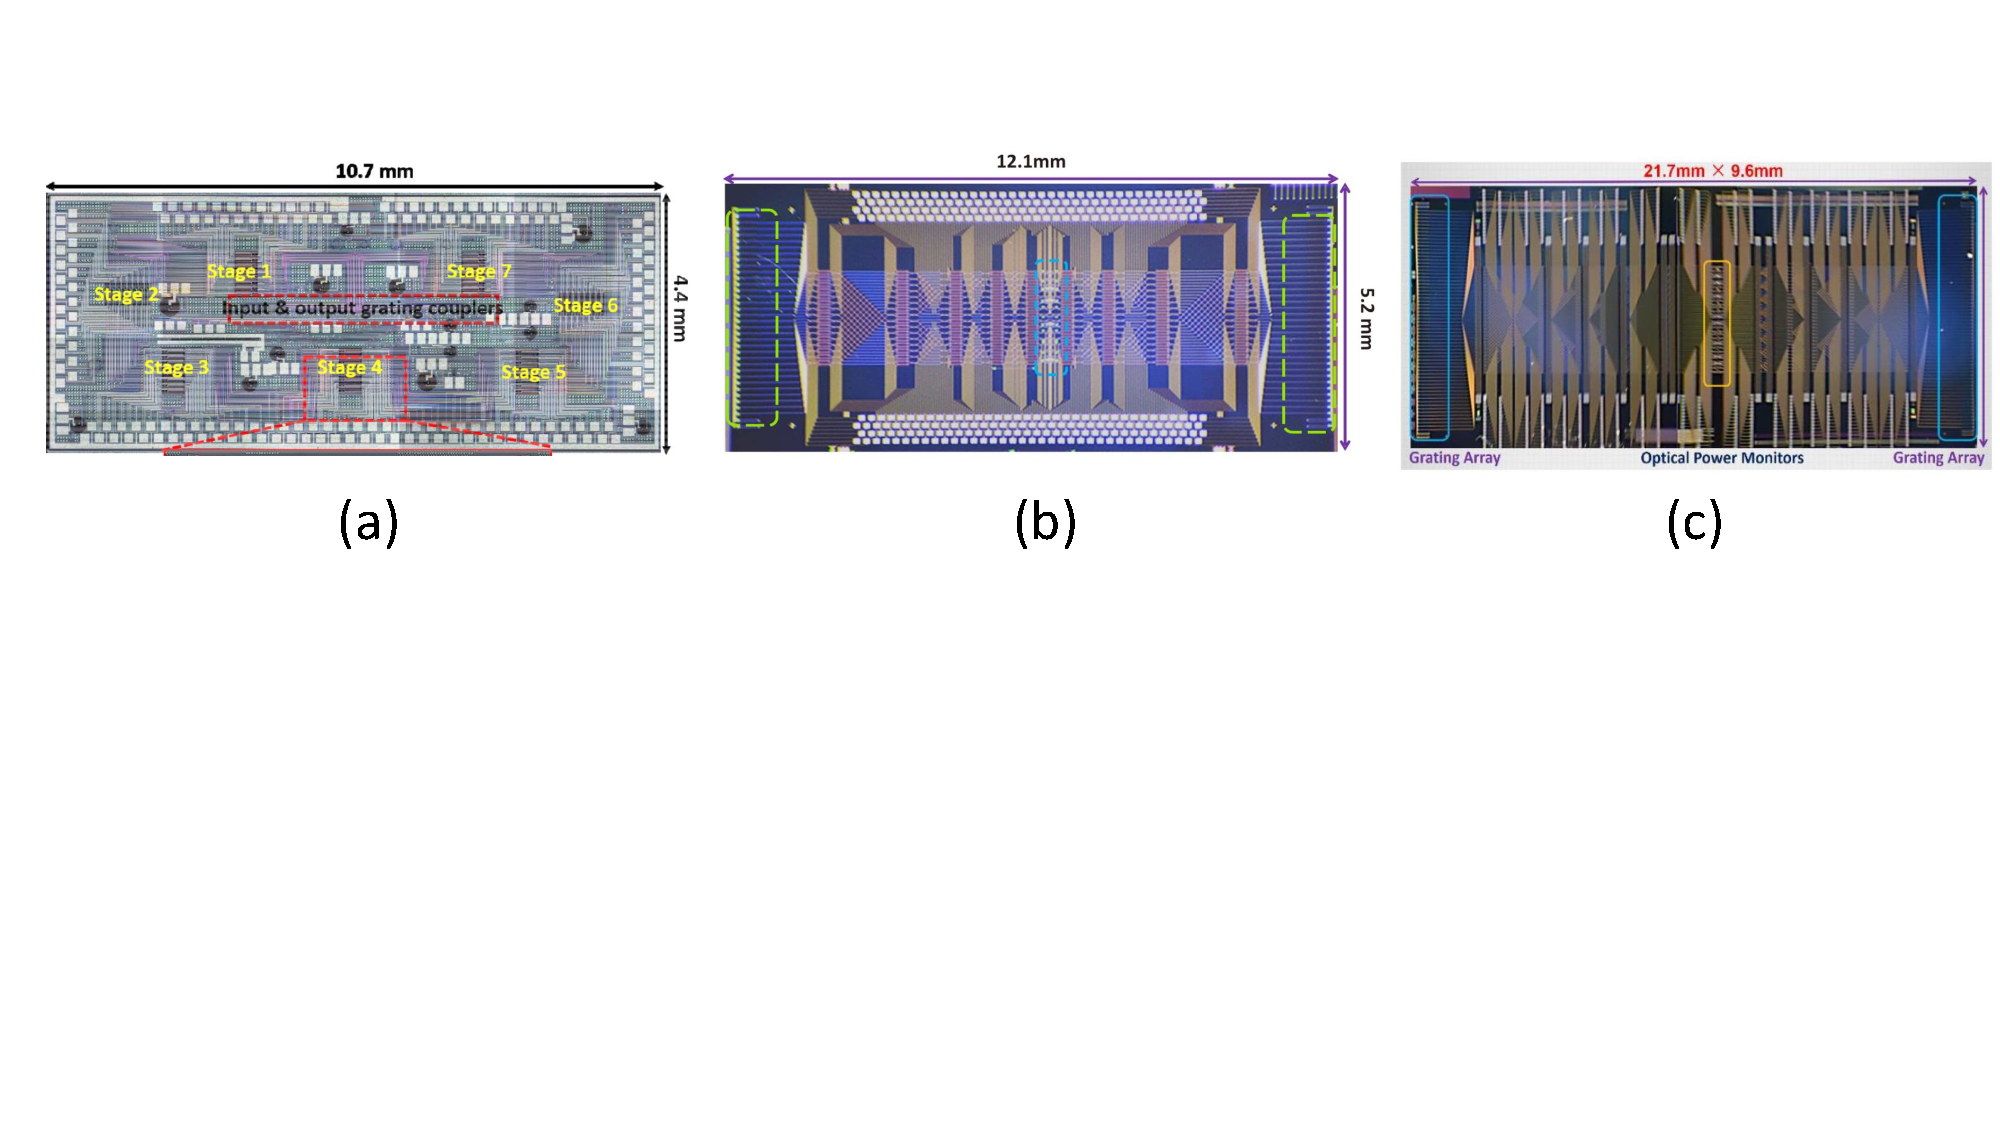
\includegraphics[clip, trim=0cm 8cm 0cm 1cm,width=15cm]{Chapter5/CH_5_fig1.pdf}
\caption{(a) (b) (c)}
\end{figure}






%%%%%%%%%%%%%%%%%%%%%%%%%%  Photo-conductance  %%%%%%%%%%%%%%%%%%%%%%%%%%
\section{Photo-conductance effect}

\begin{figure}[t!]
\centering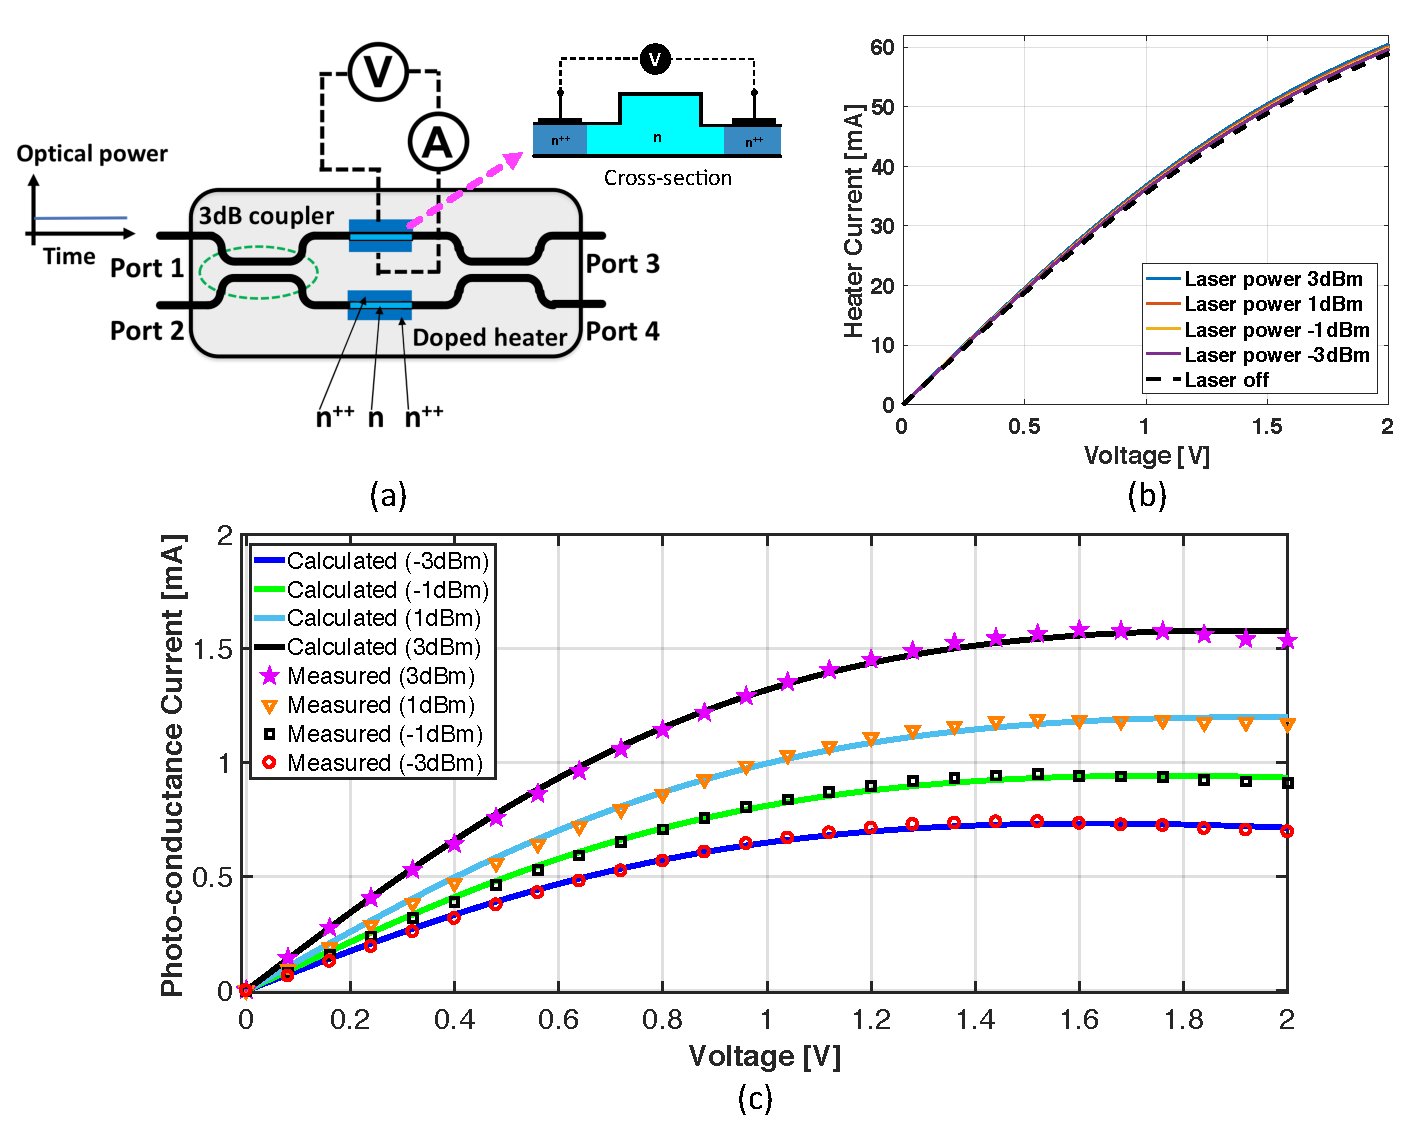
\includegraphics[width=12.5cm]{Chapter5/fig1_MB_v2.pdf}
\caption{(a) Schematic of a 2$\times$2 MZI element with doped-waveguide heater (inset shows the cross-section of the waveguide). An external optical source along with voltage and current meters are used to measure the PC effect. (b) Measured I-V curves of the heater at different input optical power. (c) Calculated (solid) and measured (markers) photo-conductance current , $\Delta I$, at different optical powers and bias voltages.}
\end{figure}

Figure 1(a) shows a schematic of the 2$\times$2 MZI element in our switch equipped with two doped heaters that are used as thermo-optic phase shifters. Each waveguide arm of the MZI is directly doped in a $n^{++}$--$n$--$n^{++}$ configuration \cite{Streshinsky}. To measure the photo-conductance effect, a variable optical power at 1550nm is injected into one of the ports of the MZI element, and a voltage sweep across the heater is performed while recording the heater current. The I-V curve of this doped heater in the absence of optical power follows the nonlinear model of an ohmic resistor due to the self-heating \cite{Bahadori_Self_heating} described by
%
\begin{equation}
\label{eq1}
I(t) = \frac{V(t)}{R_0} \, \frac{2}{1+\sqrt{1+K_v \, V(t)^2}}
\end{equation}
%
where $R_0$ is the linear resistivity at low voltage (or more precisely at low ohmic power) and $K_v$ is the thermal nonlinearity coefficient. The second factor in Eq. (\ref{eq1}) describes the deviation from the linear Ohm's law. The dashed curve in Fig. 1(b) shows the measured I-V response of one of the MZI heating elements in the \textit{absence} of injected optical power. The parameters of the heater are extracted as $R_0 = $  25.824 $\Omega$ and $K_v = $ 0.404 V$^{-2}$. The solid curves in Fig. 1(b) correspond to the measured I-V curves of the heater in the \textit{presence} of optical power inside the waveguide. As it is seen, in the presence of light the I-V curve of the heater moves up slightly showing less resistivity and higher current (\textit{photo-conductance effect}). 

To explain this, we note that the linear and/or nonlinear absorption of light inside the doped waveguide will generate extra electrons and holes that contribute a change to the ohmic conductivity as
%
\begin{equation}\label{eq2}
\sigma = \sigma_0 + \Delta \sigma = \sigma_0 \, (1+K_{p_1} P_\text{wg} + K_{p_2} P_\text{wg}^2)
\end{equation}
%
where $K_{p_1}$ (in units of mW$^{-1}$) is associated with the linear process and $K_{p_2}$ (in units of mW$^{-2}$) is associated with the two-photon absorption\cite{Zhou_PC}, $\sigma_0$ is the original conductivity, and $P_\text{wg}$ is the optical power inside the waveguide (in units of mW). A change in the conductivity subsequently affects the two parameters of the I-V model in Eq. (\ref{eq1}) according to
%
\begin{equation}\label{eq3}
R_0^\prime \approx \frac{R_0}{1+\delta} \quad , \quad K_v^\prime \approx K_v \, (1+\delta)^2 \approx K_v \, (1+2\delta) .
\end{equation}
%
where $\delta = K_{p_1} P_\text{wg} + K_{p_2} P_\text{wg}^2$ is the relative change in the ohmic conductivity of the heater (see Appendix I in \cite{Bahadori_Self_heating}). This is observed in Fig. 1(b) with the slight increase in the I-V curve of the heater for increased input optical power. In table \ref{table1}, $R_0^\prime$, and $K_v^\prime$ are extracted for all the five cases in Fig. 2(b) using a nonlinear least squares fitting. The value of parameter $\delta$ is then evaluated for each case using an average value of
%
\begin{equation}
%\delta \approx \sqrt{\frac{K_v^\prime}{K_v} \times \frac{R_0^\prime}{R_0}} -1 \, .
\delta \approx \frac{1}{2}\left[\sqrt{\frac{K_v^\prime}{K_v}} + \frac{R_0}{R_0^\prime}\right] -1
\end{equation}
%
As expected, increasing the input optical power will lead to an increase in $K_v$ (9.4\%) and $\delta$, while $R_0$ shows a decreasing trend (4.3\%). The value of $R_0 \times K_v$ also exhibits a steady increase of 4.6\% which is close to the decrease rate in $R_0$ and is in  good agreement with Eq. (\ref{eq3}).

By substituting the parameters of Eq. (\ref{eq3}) in the I-V equation Eq. (\ref{eq1}) the following result for the photo-conductance current $\Delta I$ = $I(P_{wg}) - I(P=0)$ is obtained:
%
\begin{equation}\label{eq4}
\Delta I = 2V \left[\frac{1}{R_0^\prime} \, \frac{1}{1+\sqrt{1+K_v^\prime \, V^2}} - \frac{1}{R_0} \, \frac{1}{1+\sqrt{1+K_v \, V^2}} \right] .
\end{equation}
%
Note that even if $K_v \rightarrow 0$, the photo-conductance current can exist, however, the $\Delta I-V$ curve will be linear. The deviation from a linear characteristic is mainly due to the $K_v$ factors that represent the thermal self-heating of the waveguide.
Figure 1(c) plots the theoretically calculated and experimentally measured photo-conductance current, $\Delta I$, indicating a good agreement. A clear dependence on the optical power at any bias voltage (higher optical power results in higher current) is observed, which can be used as a means to monitor the optical power inside each arm of the MZI by sensing the amount of the extra current.


\begin{table}[t] 
\footnotesize
\centering
\caption{Extracted heater parameters in the absence and presence of optical power inside the waveguide.}
\begin{tabular}{lccccc|c}
\hline
\textbf{P$_\text{laser}$ (dBm)} & \textbf{$-\infty$} & \textbf{-3} & \textbf{-1} & \textbf{1} & \textbf{3} & \textbf{Trend} \\ \midrule
\textbf{$R_0 \, (\Omega)$} & 25.824 & 25.2513 & 25.1244 & 24.9837 & 24.7188 & 4.3\% decrease \\ \hdashline
\textbf{$K_v \, (\textrm{V}^{-2})$} & 0.404 & 0.4264 & 0.4294 & 0.4321 & 0.4418 & 9.4\% increase \\ \hdashline
\textbf{$R_0 \times K_v$} & 10.4329 & 10.7672 & 10.7884 & 10.7955 & 10.92 & 4.6\% increase \\  \hdashline
\textbf{$\delta$} & 0 & 0.025 & 0.03 & 0.034 & 0.045 & increase \\ \bottomrule
\end{tabular}
\label{table1}
\end{table}




\subsection{Response time of the photo conductance effect}

\begin{figure}[b]
\vspace{-4mm}
\centering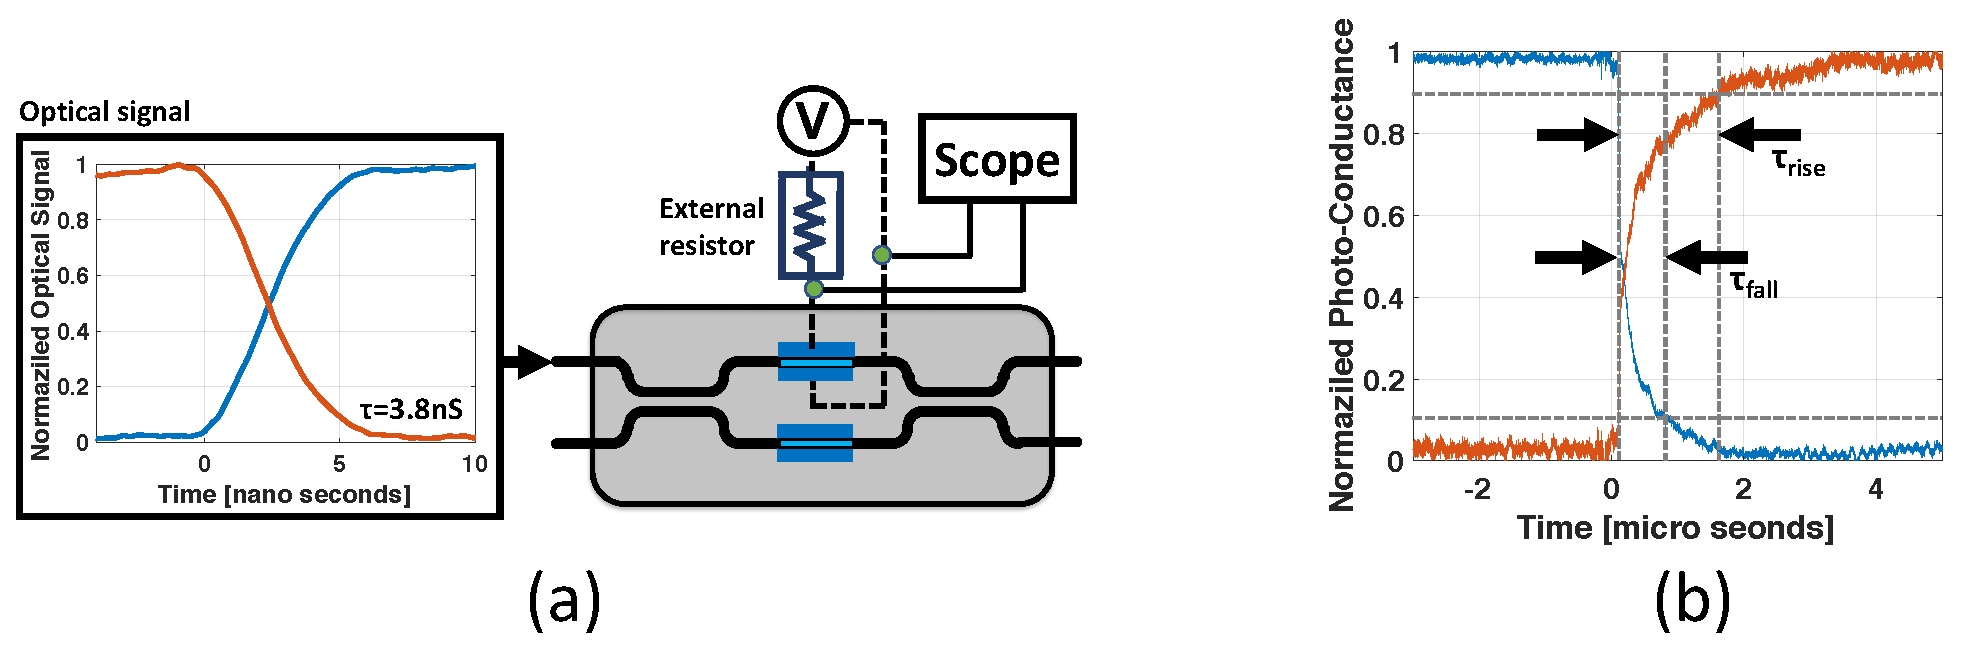
\includegraphics[scale=0.4]{Chapter5/fig2_trans_3}
\caption{(a) Schematic of the photo-conductance transient measurement. (b) Transient response of an optical step function signal. The blue curve corresponds to the rising edge of optical power and the red corresponds to the falling edge of optical power.}

\end{figure}

The transient response time of the PC effect is essential for the calibration procedure and hardware development since it determines the necessary wait time for the effect to reach the steady state. 

As illustrated in Fig. 2(a), a continuous square optical signal is injected into one of the MZI element ports while a steady bias voltage is applied through an external serial resistor. As shown here, the rise and fall times of input optical signal is measured to be 3.8 nsec. 
%
A scope is connected in parallel to the doped heater of the MZI to measure the voltage drop as a function of time. Due to the PC effect, as the optical power increases the resistivity value of the doped heater decreases and the voltage also decreases. Figure 2(b) shows a normalized measured transient response (read out voltage across the heater) for both the rising and falling edges of the optical signal. The blue curve (falling edge of voltage) corresponds to the low-to-high optical step function (rising edge of the optical power)  with a rise-time response $\uptau_{rise}$ (10\% to 90\% change) of 0.7 $\mu$sec and the red curve (rising edge of voltage) corresponds to the high-to-low optical step function (falling edge of the optical power) with a fall-time response $\uptau_{fall}$ (90\% to 10\% change) of 1.5 $\mu$sec. Clearly, these rise and fall times are much larger than the rise and fall times of the input optical pulses. These results correspond to a frequency bandwidth of $\sim100$ KHz which has also been reported in\cite{Dong_PC}.














%%%%%%%%%%%%%%%%%%%%%%%%%  Calibration algorithm  %%%%%%%%%%%%%%%%%%%%%%%%%



\section{Photo-conductance calibration}

\subsection{Calibration algorithm}
The topology-agnostic calibration algorithm based on the PC effect is outlined in the psuedo-code of Fig. 3(a). The algorithm iterates through every MZI element in the switch topology (1$\times$N, N$\times$1 and N$\times$N) to find the necessary control bias voltages over the phase-shifters to set it for the CROSS or BAR states. Figure 3(b) illustrates a generic topology of cascaded MZI elements: ``A'', ``B'', ``C'' and ``D'' in a switch design. The algorithm performs the calibration in an iterative manner starting with the MZI elements connected to the optical I/O interface. The algorithm first establishes an optical path to the MZI element under calibration. In the example of Fig. 3(b), if MZI ``A" is connected directly to the optical I/O port of the switch, no further action is required because the optical path is pre-established. Whereas for the inner MZI elements in the switch topology, the optical path is established based on the previously calibrated MZIs.


\begin{figure}[ht!]
\centering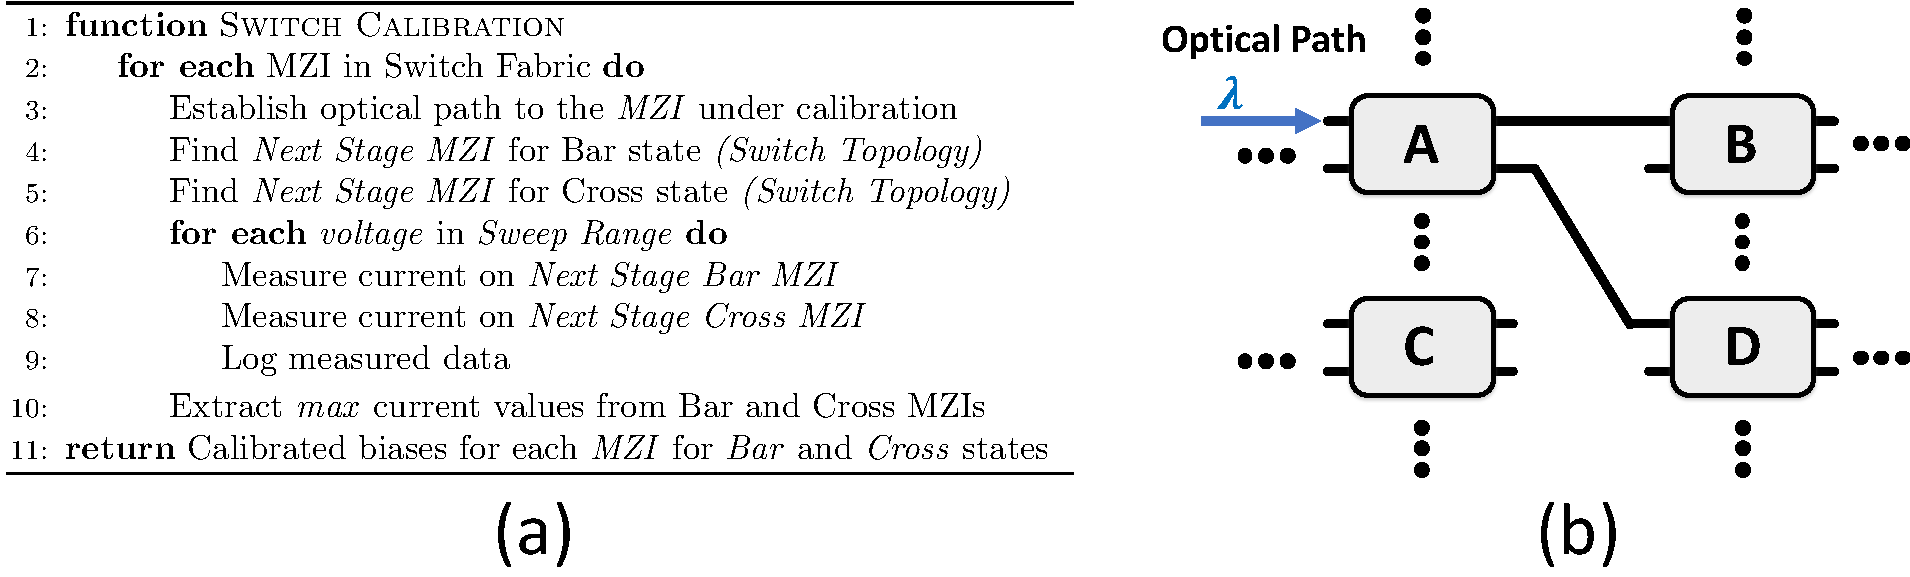
\includegraphics[width=13.5cm]{Chapter5/fig3_alg}
\caption{(a) Psuedo-code of the calibration algorithm. (b) A generic switch section topology of cascaded MZIs. }
\end{figure}

In the next step, the algorithm identifies the two MZIs optically wired to the MZI under calibration within the optical path. In the example of Fig. 3(b),  MZI ``B" and ``D" are used to monitor the PC excess current in the calibration procedure of MZI ``A". In this configuration and based on the optical path, when the maximum optical power is propagating to MZI ``B", MZI ``A" is in BAR state, and when the maximum optical power is propagating to MZI ``D", MZI ``A" is in the CROSS state. To identify these states, the control voltage is swept over MZI ``A" while 1V over the doped-heaters is applied on the MZI ``B" and ``D" and the source's current is logged. Due to the PC effect, the current change is directly related to the optical power. The bias points of MZI ``A" at the maximum current values are measured from the monitoring MZIs ``B"  and ``D" indicating the calibrated values for the BAR and CROSS states, respectively. At the end of the procedure, the algorithm returns a look-up table with each element's associated CROSS and BAR control biases.  

\subsection{Calibration of a 4$\times$4 switch}
The calibration based on the PC effect is performed on a SiP non-blocking 4$\times$4 switch illustrated in the Fig. 4(a) (the layout is outlined in \cite{Qixiang_smart_routing}). The switch consists of eight bi-directional optical I/O ports where the left-sided are denoted as inputs and the right-sided as outputs, and six optically wired 2$\times$2 MZI elements. Each MZI is equipped with two doped heaters to control the state of the switch in a push-pull approach \cite{Yishen_Push_Pull}, however, here we use only the top arm doped heater in the calibration process. 

\begin{figure}[t!]
\centering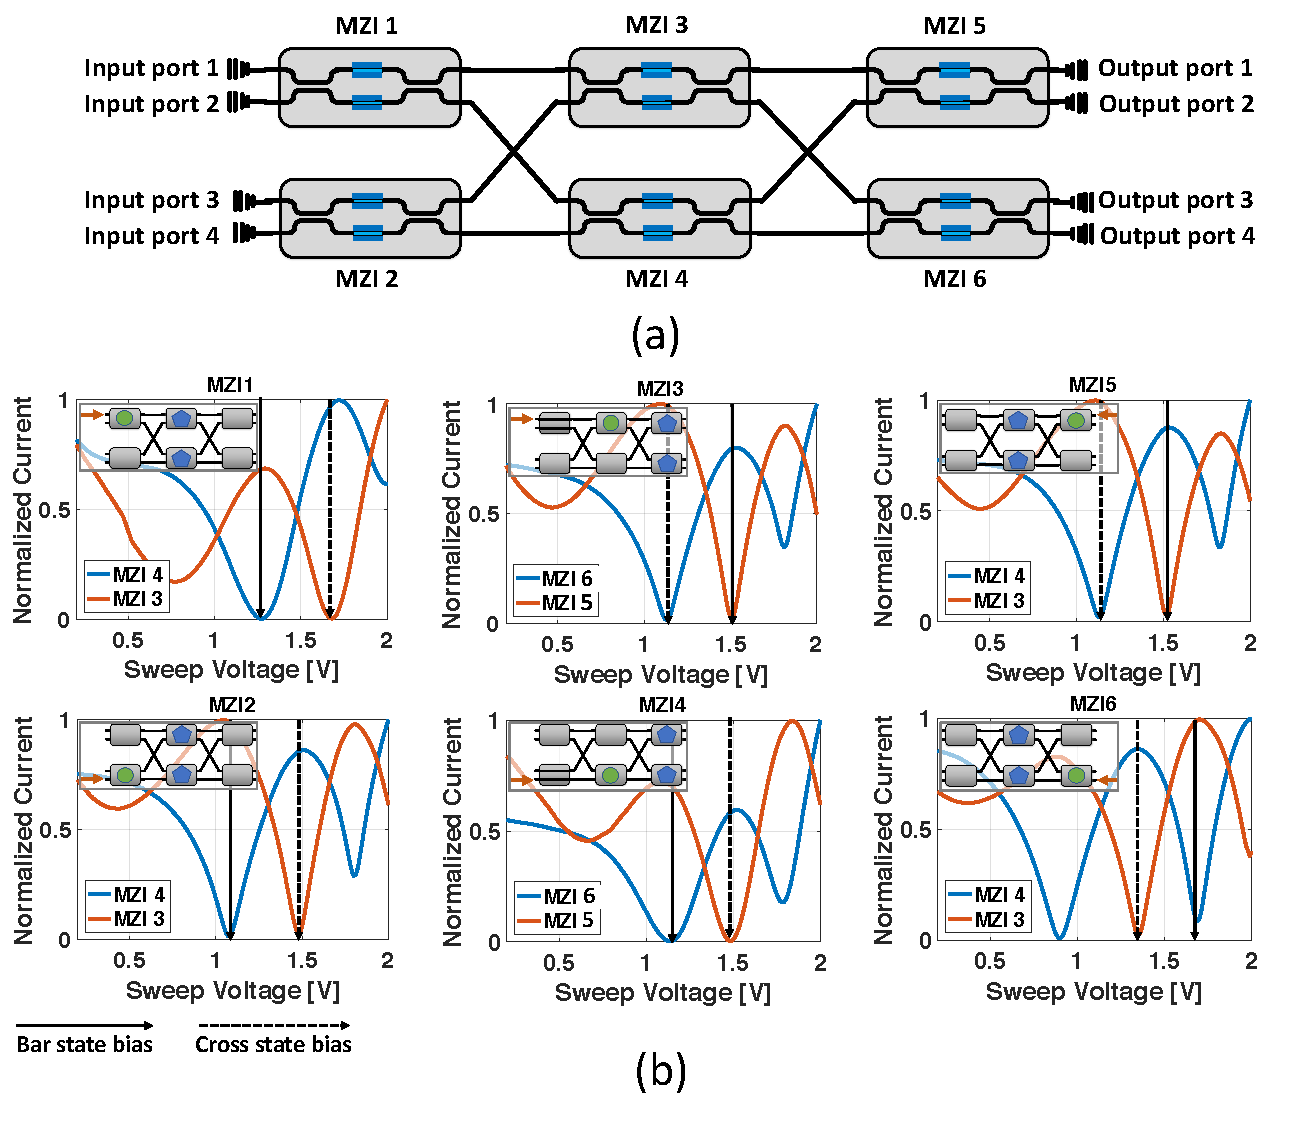
\includegraphics[width=13.5cm]{Chapter5/fig4_PC_switch_2}
\vspace{-4mm}
\caption{(a) Schematic of a the 4$\times$4 switch consisting of six MZI elements. (b) Measured PC calibration results of six MZI elements in 4$\times$4 non-blocking topology. Each plot corresponds to a single MZI element and the curves are measured currents of the proceeding MZI elements with optical path. The insets show the switch topology with the green circles corresponding to the calibrated element and the two blue pentagon shapes corresponds to the monitored elements.}
\end{figure}

The measured calibration results of each MZI element in the switch are shown in Fig. 4(b). The calibration is performed sequentially from MZI1-MZI6. The curves in the plots represent the normalized sourced current from the monitoring MZIs while 1V bias is applied and sweeping the MZI under calibration between 0-2V. The plots' insets represent the calibration setups during the algorithm process where the orange arrow is the optical source (1550nm) input, the green circle is the MZI under calibration and the two blue pentagons shapes represent the monitoring MZIs. Based on the algorithm procedure, the first MZIs to be calibrated are the ones connected to the optical I/O of the switch. Starting from MZI1, the optical signal is coupled through the top input of the 2$\times$2 element, therefore, maximum sourced current on MZI3 indicates the BAR state and the maximum current at MZI4 (or minimum at MZI3) indicates the CROSS state for MZI1. Considering the optical coupling port in the calibration result of MZI2, maximum current at MZI3 indicates the CROSS state for MZI2 while maximum current at MZI4 indicates BAR state for MZI2. 


The calibration of the inner MZIs (3 and 4), requires information of the previously calibrated elements. Continuing with MZI3, the algorithm sets the optical path by applying appropriate control voltage for a BAR state on MZI1 (inset of Fig. 4(b) - MZI3), and utilizing MZI5 and MZI6 as monitoring elements. Similarly, the optical path to MZI4 was set by biasing MZI2 to the BAR state. Lastly, the calibration of MZI5 and MZI6 is implemented by coupling the optical signal through the output ports while MZI3 and MZI4 are used as the monitoring elements.  




The vertical solid and dashed arrows in Fig. 4(b) indicate the calibrated control voltages to set each MZI element to the BAR and CROSS states, respectively. In the next section, the calibrated results are used to control the 4$\times$4 switch, and all possible routing configurations are evaluated for insertion loss, extinction ratio and the quality of optical data switching performances. 


Note that a change in the input optical power will modify the bias voltages necessary to put a 2$\times$2 switch element in the Bar or Cross state. However, by combining Eq. \mbox{(\ref{eq1})} through Eq. \mbox{(\ref{eq3})} it is possible to add a corrective term to the bias voltages after the initial characterization of the heaters is done. The variable that remains unchanged is the required change of temperature of waveguide and it is linearly proportional to the required ohmic power. Therefore, the bias voltages measured at a particular optical power will have to decrease if the optical power is increased and vice versa.



% Please add the following required packages to your document preamble:
% \usepackage[table,xcdraw]{xcolor}
% If you use beamer only pass "xcolor=table" option, i.e. \documentclass[xcolor=table]{beamer}
% \begin{table}[ht]
% \footnotesize
% \centering
% \begin{tabular}{l|c|c|}
% \cline{2-3}
% & \multicolumn{1}{l|}{\textbf{Bar state [V]} } & \multicolumn{1}{l|}{\textbf{Cross state [V]} } \\ \hline
% \rowcolor[HTML]{C0C0C0} 
% \multicolumn{1}{|l|}{\cellcolor[HTML]{C0C0C0}\textbf{MZI 1}} & 1.25 & 1.64 \\ \hline
% \multicolumn{1}{|l|}{\textbf{MZI 2}}                         & 1.09 & 1.51 \\ \hline
% \rowcolor[HTML]{C0C0C0} 
% \multicolumn{1}{|l|}{\cellcolor[HTML]{C0C0C0}\textbf{MZI 3}} & 1.49 & 1.10 \\ \hline
% \multicolumn{1}{|l|}{MZI 4}                                  & 1.13 & 1.47 \\ \hline
% \rowcolor[HTML]{C0C0C0} 
% \multicolumn{1}{|l|}{\cellcolor[HTML]{C0C0C0}\textbf{MZI 5}}          & 1.55 & 1.18 \\ \hline
% \multicolumn{1}{|l|}{\textbf{MZI 6}}                                & 1.74 & 1.40 \\ \hline
% \end{tabular}
% \caption{Extracted calibrated biases of each MZI element in the 4x4 switch for cross and bar states}
% \end{table}


% \begin{figure}[ht!]
% \centering\includegraphics[width=3.5cm]{fig5_biases}
% \caption{Extracted calibrated biases of each MZI element in the 4x4 switch for cross and bar states}
% \end{figure}





%%%%%%%%%%%%%%%%%%%%%%%%%  Discussion  %%%%%%%%%%%%%%%%%%%%%%%%%
\section{Calibration evaluation}
\subsection{Experimental setup}



\begin{figure}[t]
\centering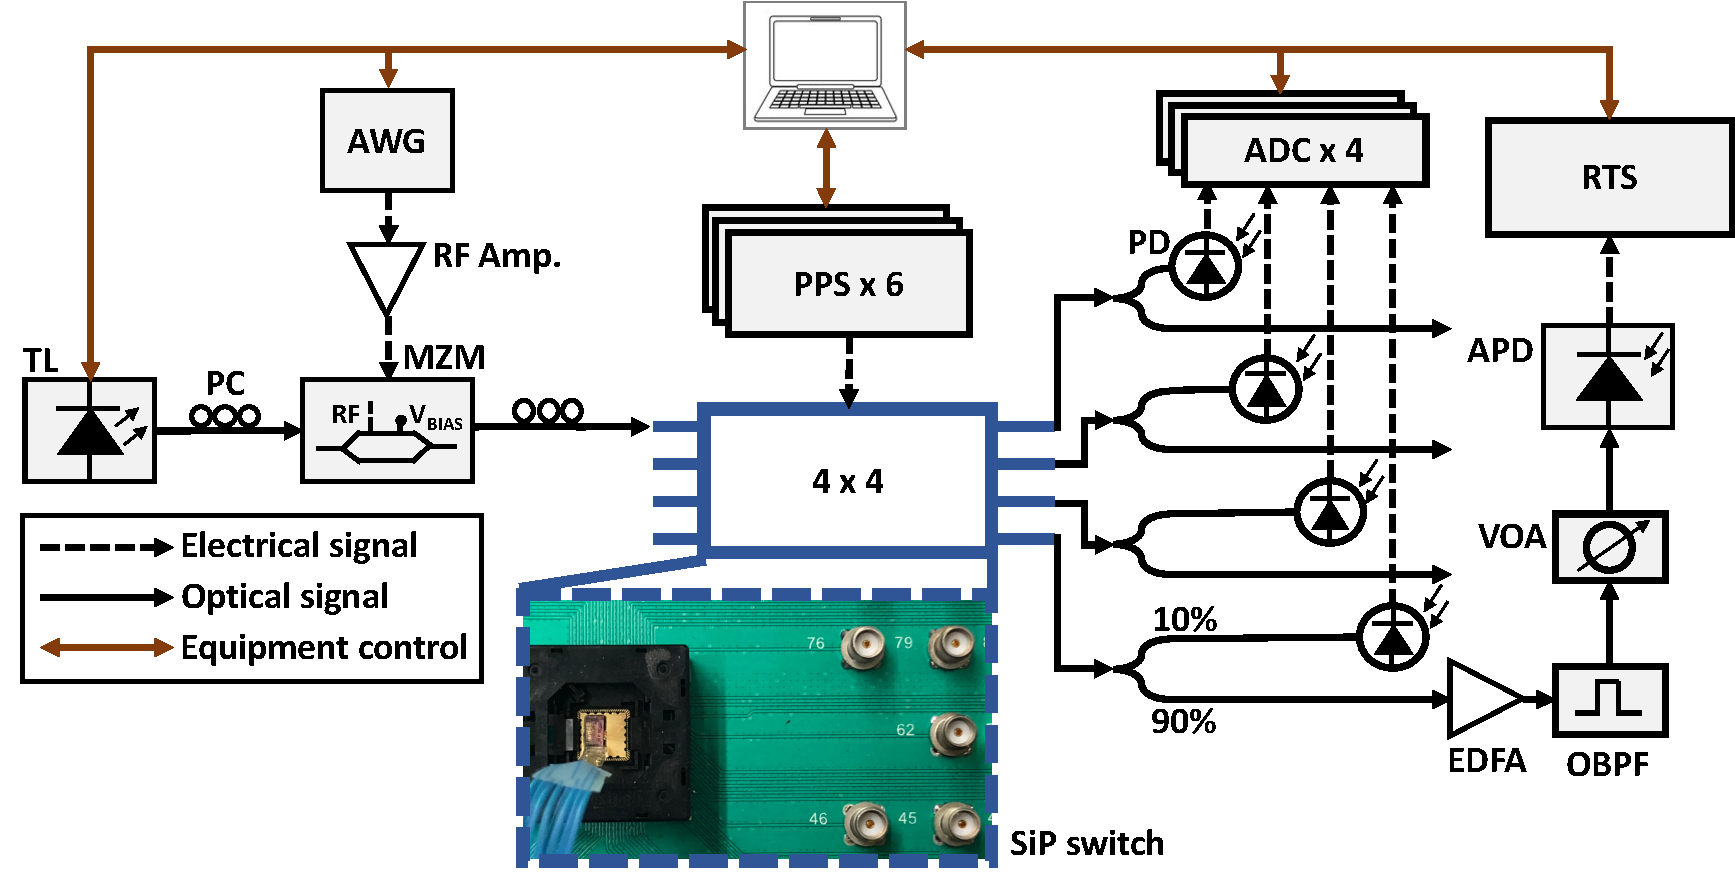
\includegraphics[width=13cm]{Chapter5/fig6_experimental}
\caption{\label{fig:setup}Schematic of the experimental setup. The setup consists of a packaged SiP switch, central control computer and the following equipment: control Arbitrary Waveform Generator (AWG), Tunable Laser (TL), Polarization Controller (PC), Mach-Zehnder Modulator (MZM), Precise Power Supply (PPS), Photo-detector (PD), Analog-to-Digital Converter (ADC), Erbium Doped Fiber Amplifier (EDFA), Optical Bandpass Filter (OBPF), Variable Optical Attenuator (VOA), Avalanche Photo-diode (APD) and Real-Time Scope (RTS).}

\end{figure}





The experimental setup is developed to verify the results of the PC calibration against calibration using external PDs, as well as to evaluate the performance of the switch as a system. Fig. \ref{fig:setup} shows a schematic of the experimental setup with the SiP 4$\times$4 switch in the center. The switch is wire-bonded on a chip carrier and mounted on a breakout printed-circuit-board to allow convenient access to the doped phase shifters of the MZI elements. An array of eight fibers is aligned and glued on top of grating couplers for optical I/O interface. 

The PC calibration algorithm is implemented in the central control computer in Python and serially interfaced to six PPSs (Keithley 2280). The PPSs are used to supply control voltages and to allow the measurement of the PC current. An optical signal (1550nm) is generated using a programmable TL and coupled into the SiP switch through a polarization controller. To validate the calibrated procedure against calibration with external PDs and to measure the steady-state insertion loss and extinction ratios, the four optical output ports are coupled to an optical splitter with 10\% of the light directed to MHz range PDs (Thorlabs PDA20CS) in each case. The PDs are connected to four ADCs (NiDAQ 6363) for power readout and results plotting.

The optical transmission is carried out by programming an AWG (Keysight M8195A) to generate 4-level pulse amplitude signals (PAM4) at 12.5 Gbaud (25 Gbps). The electrical PAM signal is amplified and then used to modulate the light from the TL using a Mach-Zehnder Modulator (MZM). Digital processing (timing deskew, resampling, adaptive equalization, matched filtering, amplitude offset compensation) and bit-error rate (BER) calculations, are performed off-line using MATLAB from the received RTS (Tektronix MSO71254C) signal. At each output port 90\% of the signal is connected to an EDFA to compensate for 10dB fiber to chip coupling loss (~5dB per grating coupler). The OBPF is used to filter the amplified spontaneous emission (ASE) noise associated with the EDFA, and the VOA used to set the optical signal falling on the APD at -5dBm.


% * <browninc@tcd.ie> 2018-09-21T15:53:06.945Z:
% 
% > (PC)
% PC definied both as photo conductance and pol. controller
% 
% ^ <browninc@tcd.ie> 2018-09-21T15:53:51.480Z.


\subsection{Calibration with external photo-detectors}

\begin{figure}[t]
\centering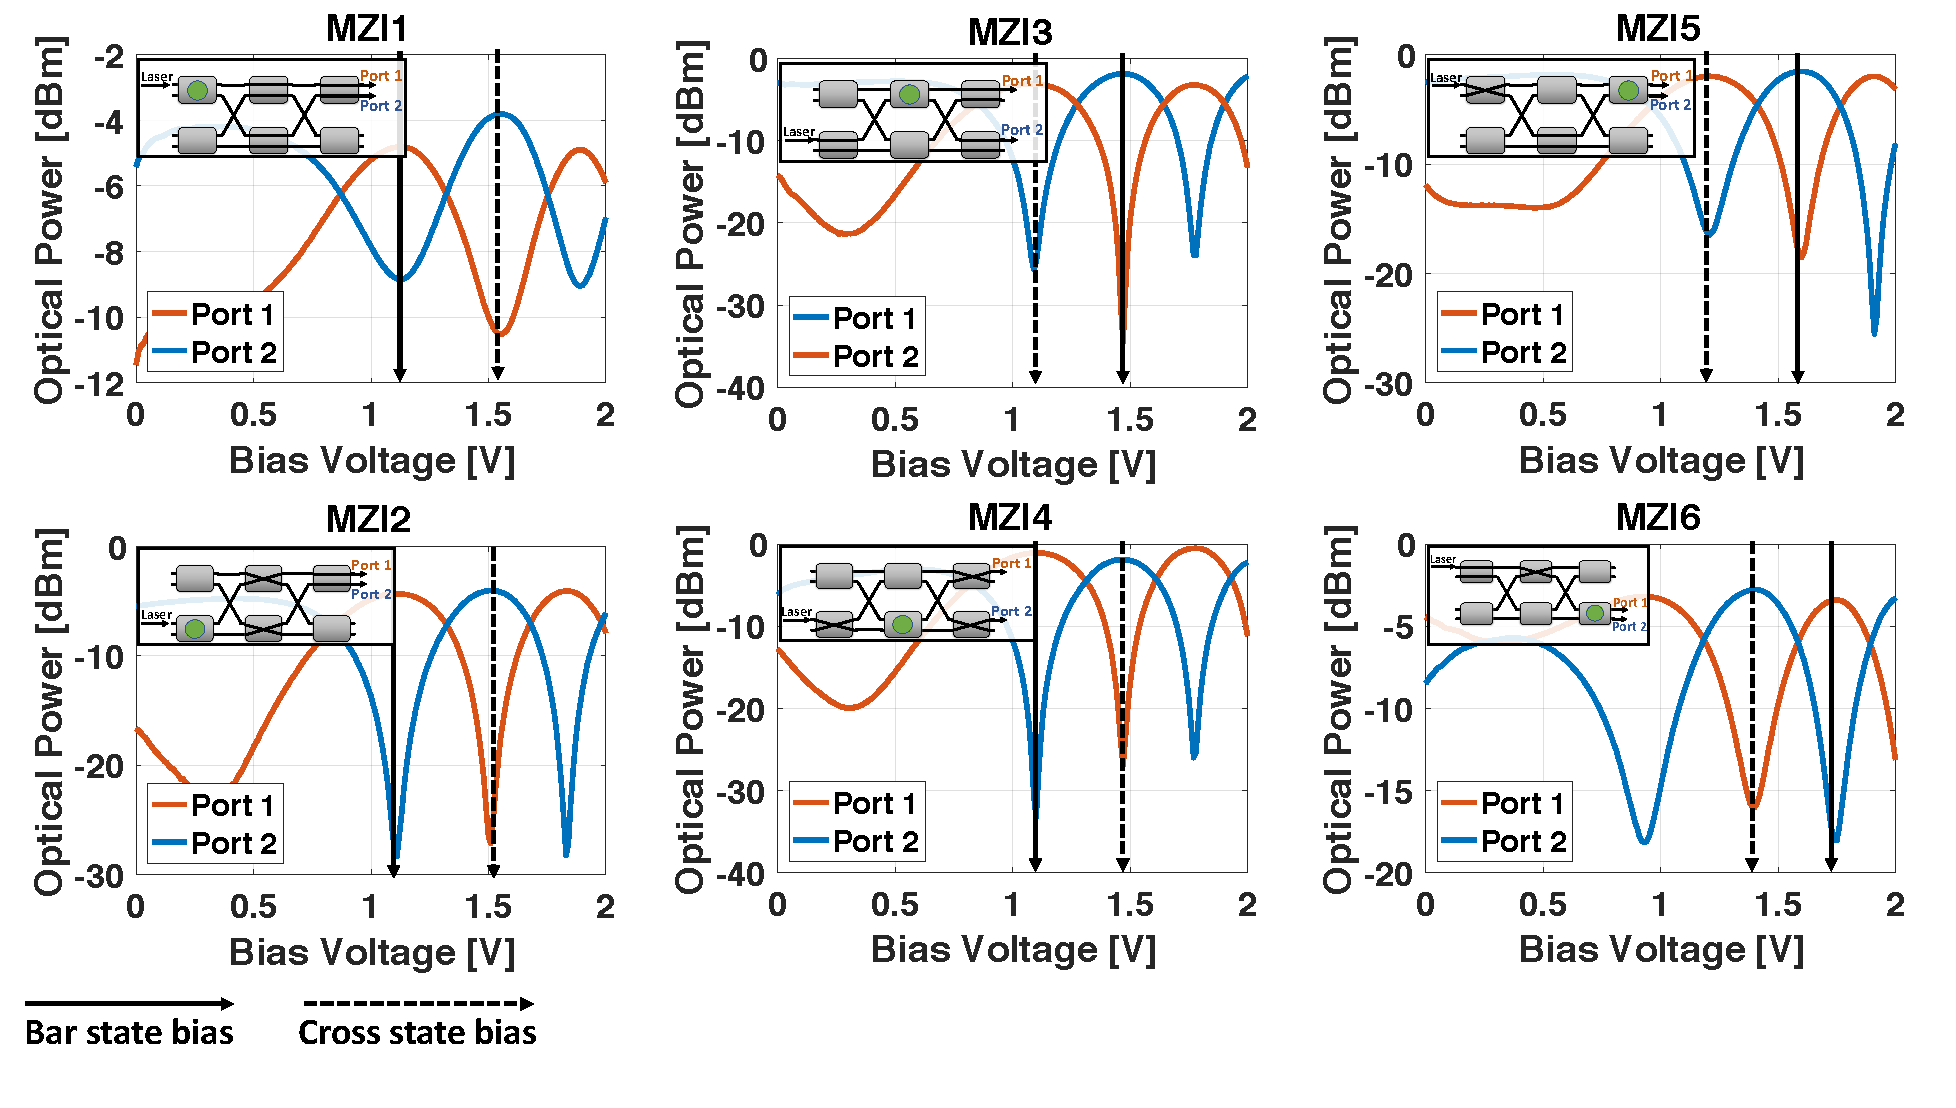
\includegraphics[width=13cm]{Chapter5/fig7_PD_charac}
\caption{Calibration of the six elements in the 4$\times$4 switch using external PDs. The insets show the MZI under calibration (marked with a green circle) and the states of supporting elements as well as the input and output optical ports.}
\end{figure}

To validate the obtained control biases for the CROSS and BAR states of each MZI element in the switch, a calibration with external PDs is performed. An optical path to the MZI under calibration and the external PDs is established using the pre-calibrated values from the PC algorithm. The plots in Fig. 6 show the measured optical power obtained from the PDs and read from the ADCs while several MZI elements set to either CROSS or BAR state and the MZI under calibration is swept again from 0-2V using the PPS. The insets of the Fig. 6 show the optical configuration of the switch during the specific MZI calibration, with the MZI marked with green circles indicate the MZI under calibration. In the case of MZI1, the optical signal is coupled from input port 1 and MZI3-5 are all set to the BAR state to guide the signal to the output ports. In this optical path configuration, MZI1 is in the BAR state when maximum optical power observed at port 1  and in the CROSS state when maximum optical power is measured at port 2. In the calibration process of MZI6, for example, MZI1 is set to BAR and MZI3 is in CROSS. In this configuration, the optical signal is guided directly to MZI6, and based on the input port to the element, maximum received power at port 1 corresponds to the BAR state and port 2 to the CROSS state. The solid and the dashed vertical arrows in Fig. 6 indicate the BAR and CROSS state of each MZI element. 


% \begin{table}[h]
% \footnotesize
% \centering
% \begin{tabular}{l|
% >{\columncolor[HTML]{C0C0C0}}c |
% >{\columncolor[HTML]{C0C0C0}}c |
% >{\columncolor[HTML]{EFEFEF}}c |
% >{\columncolor[HTML]{EFEFEF}}c |}
% \cline{2-5}
% & \multicolumn{2}{l|}{\cellcolor[HTML]{C0C0C0}\textbf{Photo-conductance}} & \multicolumn{2}{l|}{\cellcolor[HTML]{EFEFEF}\textbf{External photo-diodes}} \\ \cline{2-5}                                                                            & \textbf{Bar {[}V{]}}              & \textbf{Cross {[}V{]}}              & \textbf{Cross {[}V{]}}                & \textbf{Bar {[}V{]}}                \\ \hline
% \multicolumn{1}{|l|}{\textbf{MZI 1}}                                                & 1.25 & 1.64 & 1.27 & 1.68 \\ \hline
% \multicolumn{1}{|l|}{\cellcolor[HTML]{9B9B9B}{\color[HTML]{000000} \textbf{MZI 2}}} & 1.09 & 1.51 & 1.07 & 1.48 \\ \hline
% \multicolumn{1}{|l|}{\textbf{MZI 3}}                                                & 1.49 & 1.10 & 1.51 & 1.13 \\ \hline
% \multicolumn{1}{|l|}{\cellcolor[HTML]{9B9B9B}\textbf{MZI 4}}                        & 1.13 & 1.47 & 1.15 & 1.48  \\ \hline
% \multicolumn{1}{|l|}{\textbf{MZI 5}}                                                & 1.55 & 1.18 & 1.52 & 1.14 \\ \hline
% \multicolumn{1}{|l|}{\cellcolor[HTML]{9B9B9B}\textbf{MZI 6}}                        & 1.74 & 1.4 & 1.69 & 1.35 \\ \hline
% \end{tabular}
% \caption{Extracted calibrated biases of each MZI element using the PC calibration algorithm and external PDs}
% \end{table}

\begin{table}[b]
\footnotesize
\centering
\caption{Extracted calibrated bias values of each MZI element using the PC calibration algorithm and external PDs.}
\begin{tabular}{lcccccc}
& \multicolumn{2}{l}{\textbf{Photo-conductance}} & \multicolumn{2}{l}{\textbf{External photo-diodes}} \\
\cline{2-5} & \textbf{Bar {[}V{]}} & \textbf{Cross {[}V{]}} & \textbf{Cross {[}V{]}} & \textbf{Bar {[}V{]}} & \textbf{$\Delta$Bar {[\%]}} & \textbf{$\Delta$Cross {[\%]}} \\ \midrule
\multicolumn{1}{l}{\textbf{MZI 1}} & 1.25 & 1.64 & 1.27 & 1.68 & 2.4 & 1.58\\ \hdashline
\multicolumn{1}{l}{\textbf{MZI 2}} & 1.09 & 1.51 & 1.07 & 1.48 & 2 & 1.85 \\ \hdashline
\multicolumn{1}{l}{\textbf{MZI 3}} & 1.49 & 1.10 & 1.51 & 1.13 & 2.7 & 1.4 \\ \hdashline
\multicolumn{1}{l}{\textbf{MZI 4}} & 1.13 & 1.47 & 1.15 & 1.48 & 0.6 & 1.75 \\ \hdashline
\multicolumn{1}{l}{\textbf{MZI 5}} & 1.55 & 1.18 & 1.52 & 1.14 & 3.4 & 1.95 \\ \hdashline
\multicolumn{1}{l}{\textbf{MZI 6}} & 1.74 & 1.4 & 1.69 & 1.35 & 3.6 & 2.9 \\ \bottomrule
\end{tabular}
\end{table}


The calibration results of the six elements in the 4$\times$4 switch using the PC algorithm and the external PDs are summarized in Table 2. The obtained control bias voltages with the two approaches show a good agreement within few percent of difference. From the results in Fig. 6 it is also possible to see that the insertion loss per measured path is not significant with increased bias voltage over the doped-heater. The injected carriers through the $n^{++}$--$n$--$n^{++}$ element do not change the carrier concentration in the waveguide, hence, there is no additional carrier absorption that contribute to loss\mbox{\cite{Soref_EO}}.



\subsection{Extinction ratio and insertion loss}

\begin{table}[t] 
\caption{Six MZI states for all possible routing configuration "input port"$\rightarrow$ "output port". States notations: "B"-BAR, "C"-CROSS and "-"-no bias.}
\begin{footnotesize}
\begin{adjustbox}{center}
\begin{tabular}{@{}llll@{}}\centering
\begin{tabular}{@{}cc@{}}\toprule
\begin{tabular}{@{}c@{}}\textbf{MZI\#}$\rightarrow$\\\hdashline $\downarrow$\textbf{Routing}\end{tabular} & \textbf{[1,2,3,4,5,6]} \\ \midrule
%\textbf{1}$\rightarrow$\textbf{1} & [C,-,-,B,C,-] \\ \hdashline
\textbf{1}$\rightarrow$\textbf{1} & [B,-,B,-,B,-] \\ \hdashline
%\textbf{1}$\rightarrow$\textbf{2} & [C,-,-,B,B,-] \\ \hdashline
\textbf{1}$\rightarrow$\textbf{2} & [B,-,B,-,C,-] \\ \hdashline
%\textbf{1}$\rightarrow$\textbf{3} & [C,-,-,C,-,C] \\ \hdashline
\textbf{1}$\rightarrow$\textbf{3} & [B,-,C,-,-,B] \\ \hdashline
%\textbf{1}$\rightarrow$\textbf{4} & [C,-,-,C,-,B] \\ \hdashline
\textbf{1}$\rightarrow$\textbf{4} & [B,-,C,-,-,C] \\ \bottomrule

\end{tabular}
\begin{tabular}{@{}cc@{}}\toprule
\begin{tabular}{@{}c@{}}\textbf{MZI\#}$\rightarrow$\\\hdashline $\downarrow$\textbf{Routing}\end{tabular} & \textbf{[1,2,3,4,5,6]} \\ \midrule
%\textbf{2}$\rightarrow$\textbf{1} & [B,-,-,B,C,-] \\ \hdashline
\textbf{2}$\rightarrow$\textbf{1} & [C,-,B,-,B,-] \\ \hdashline
%\textbf{2}$\rightarrow$\textbf{2} & [B,-,-,B,B,-] \\ \hdashline
\textbf{2}$\rightarrow$\textbf{2} & [C,-,B,-,C,-] \\ \hdashline
%\textbf{2}$\rightarrow$\textbf{3} & [B,-,-,C,-,C] \\ \hdashline
\textbf{2}$\rightarrow$\textbf{3} & [C,-,C,-,-,B] \\ \hdashline
%\textbf{2}$\rightarrow$\textbf{4} & [B,-,-,C,-,B] \\ \hdashline
\textbf{2}$\rightarrow$\textbf{4} & [C,-,C,-,-,C] \\ \bottomrule
\end{tabular}
\begin{tabular}{@{}cc@{}}\toprule
\begin{tabular}{@{}c@{}}\textbf{MZI\#}$\rightarrow$\\\hdashline $\downarrow$\textbf{Routing}\end{tabular} & \textbf{[1,2,3,4,5,6]} \\ \midrule
%\textbf{3}$\rightarrow$\textbf{1} & [-,C,-,C,C,-] \\ \hdashline
\textbf{3}$\rightarrow$\textbf{1} & [-,B,C,-,B,-] \\ \hdashline
%\textbf{3}$\rightarrow$\textbf{2} & [-,C,-,C,B,-] \\ \hdashline
\textbf{3}$\rightarrow$\textbf{2} & [-,B,C,-,C,-] \\ \hdashline
%\textbf{3}$\rightarrow$\textbf{3} & [-,C,-,B,-,C] \\ \hdashline
\textbf{3}$\rightarrow$\textbf{3} & [-,B,B,-,-,B] \\ \hdashline
%\textbf{3}$\rightarrow$\textbf{4} & [-,C,-,B,-,B] \\ \hdashline
\textbf{3}$\rightarrow$\textbf{4} & [-,B,B,-,-,C] \\ \bottomrule

\end{tabular}
\begin{tabular}{@{}cc@{}}\toprule
\begin{tabular}{@{}c@{}}\textbf{MZI\#}$\rightarrow$\\\hdashline $\downarrow$\textbf{Routing}\end{tabular} & \textbf{[1,2,3,4,5,6]} \\ \midrule
%\textbf{4}$\rightarrow$\textbf{1} & [-,B,-,C,C,-] \\ \hdashline
\textbf{4}$\rightarrow$\textbf{1} & [-,C,C,-,B,-] \\ \hdashline
%\textbf{4}$\rightarrow$\textbf{2} & [-,B,-,C,B,-] \\ \hdashline
\textbf{4}$\rightarrow$\textbf{2} & [-,C,C,-,C,-] \\ \hdashline
%\textbf{4}$\rightarrow$\textbf{3} & [-,B,-,B,-,C] \\ \hdashline
\textbf{4}$\rightarrow$\textbf{3} & [-,C,B,-,-,B] \\ \hdashline
%\textbf{4}$\rightarrow$\textbf{4} & [-,B,-,B,-,B] \\ \hdashline
\textbf{4}$\rightarrow$\textbf{4} & [-,C,B,-,-,C] \\\bottomrule
\end{tabular}
\end{tabular}
\end{adjustbox}
\end{footnotesize}

\end{table}

%% original table 
% \begin{table}[t] 
% \begin{footnotesize}
% \begin{adjustbox}{center}
% \begin{tabular}{@{}llll@{}}\centering
% \begin{tabular}{@{}cc@{}}\toprule
% \begin{tabular}{@{}c@{}}\textbf{MZI\#}$\rightarrow$\\\hdashline $\downarrow$\textbf{Routing}\end{tabular} & \textbf{[1,2,3,4,5,6]} \\ \midrule
% \textbf{1}$\rightarrow$\textbf{1} & [B,-,B,-,B,-] \\ \hdashline
% \textbf{1}$\rightarrow$\textbf{1} & [C,-,-,B,C,-] \\ \hdashline
% \textbf{1}$\rightarrow$\textbf{2} & [B,-,B,-,C,-] \\ \hdashline
% \textbf{1}$\rightarrow$\textbf{2} & [C,-,-,B,B,-] \\ \hdashline
% \textbf{1}$\rightarrow$\textbf{3} & [B,-,C,-,-,B] \\ \hdashline
% \textbf{1}$\rightarrow$\textbf{3} & [C,-,-,C,-,C] \\ \hdashline
% \textbf{1}$\rightarrow$\textbf{4} & [B,-,C,-,-,C] \\ \hdashline
% \textbf{1}$\rightarrow$\textbf{4} & [C,-,-,C,-,B] \\ \bottomrule
% \end{tabular}
% \begin{tabular}{@{}cc@{}}\toprule
% \begin{tabular}{@{}c@{}}\textbf{MZI\#}$\rightarrow$\\\hdashline $\downarrow$\textbf{Routing}\end{tabular} & \textbf{[1,2,3,4,5,6]} \\ \midrule
% \textbf{2}$\rightarrow$\textbf{1} & [B,-,-,B,C,-] \\ \hdashline
% \textbf{2}$\rightarrow$\textbf{1} & [C,-,B,-,B,-] \\ \hdashline
% \textbf{2}$\rightarrow$\textbf{2} & [B,-,-,B,B,-] \\ \hdashline
% \textbf{2}$\rightarrow$\textbf{2} & [C,-,B,-,C,-] \\ \hdashline
% \textbf{2}$\rightarrow$\textbf{3} & [B,-,-,C,-,C] \\ \hdashline
% \textbf{2}$\rightarrow$\textbf{3} & [C,-,C,-,-,B] \\ \hdashline
% \textbf{2}$\rightarrow$\textbf{4} & [B,-,-,C,-,B] \\ \hdashline
% \textbf{2}$\rightarrow$\textbf{4} & [C,-,C,-,-,C] \\ \bottomrule
% \end{tabular}
% \begin{tabular}{@{}cc@{}}\toprule
% \begin{tabular}{@{}c@{}}\textbf{MZI\#}$\rightarrow$\\\hdashline $\downarrow$\textbf{Routing}\end{tabular} & \textbf{[1,2,3,4,5,6]} \\ \midrule
% \textbf{3}$\rightarrow$\textbf{1} & [-,B,C,-,B,-] \\ \hdashline
% \textbf{3}$\rightarrow$\textbf{1} & [-,C,-,C,C,-] \\ \hdashline
% \textbf{3}$\rightarrow$\textbf{2} & [-,B,C,-,C,-] \\ \hdashline
% \textbf{3}$\rightarrow$\textbf{2} & [-,C,-,C,B,-] \\ \hdashline
% \textbf{3}$\rightarrow$\textbf{3} & [-,B,B,-,-,B] \\ \hdashline
% \textbf{3}$\rightarrow$\textbf{3} & [-,C,-,B,-,C] \\ \hdashline
% \textbf{3}$\rightarrow$\textbf{4} & [-,B,B,-,-,C] \\ \hdashline
% \textbf{3}$\rightarrow$\textbf{4} & [-,C,-,B,-,B] \\ \bottomrule
% \end{tabular}
% \begin{tabular}{@{}cc@{}}\toprule
% \begin{tabular}{@{}c@{}}\textbf{MZI\#}$\rightarrow$\\\hdashline $\downarrow$\textbf{Routing}\end{tabular} & \textbf{[1,2,3,4,5,6]} \\ \midrule
% \textbf{4}$\rightarrow$\textbf{1} & [-,B,-,C,C,-] \\ \hdashline
% \textbf{4}$\rightarrow$\textbf{1} & [-,C,C,-,B,-] \\ \hdashline
% \textbf{4}$\rightarrow$\textbf{2} & [-,B,-,C,B,-] \\ \hdashline
% \textbf{4}$\rightarrow$\textbf{2} & [-,C,C,-,C,-] \\ \hdashline
% \textbf{4}$\rightarrow$\textbf{3} & [-,B,-,B,-,C] \\ \hdashline
% \textbf{4}$\rightarrow$\textbf{3} & [-,C,B,-,-,B] \\ \hdashline
% \textbf{4}$\rightarrow$\textbf{4} & [-,B,-,B,-,B] \\ \hdashline
% \textbf{4}$\rightarrow$\textbf{4} & [-,C,B,-,-,C] \\\bottomrule
% \end{tabular}
% \end{tabular}
% \end{adjustbox}
% \end{footnotesize}
% \caption{Six MZI states for all possible routing configuration "input port"$\rightarrow$ "output port". States notations: "B"-BAR, "C"-CROSS and "-"-no bias.}
% \end{table}

%% end of original table

%%%%%%%%%%%%%%%%%%%%%%%%%%%%%%%%%%%%%%% end table 2

With the obtained calibrated results from the PC algorithm, the 4$\times$4 subsystem switch performance is evaluated first for the extinction ratio and the insertion loss per routing configuration. Table 3 shows MZI states used to control the switch for all possible one input to one output (\textit{input}$\rightarrow$\textit{output}) configurations. The BAR and the CROSS state are denoted with letter "B" and "C". MZI elements not participating in the routing configuration are left at 0V bias state and denoted as "-". The MZI configurations are saved as a look-up table in the central computer and applied through the PPS. At each applied routing configuration, received optical power from the four output ports are recorded. 


\begin{figure}[b!]
\centering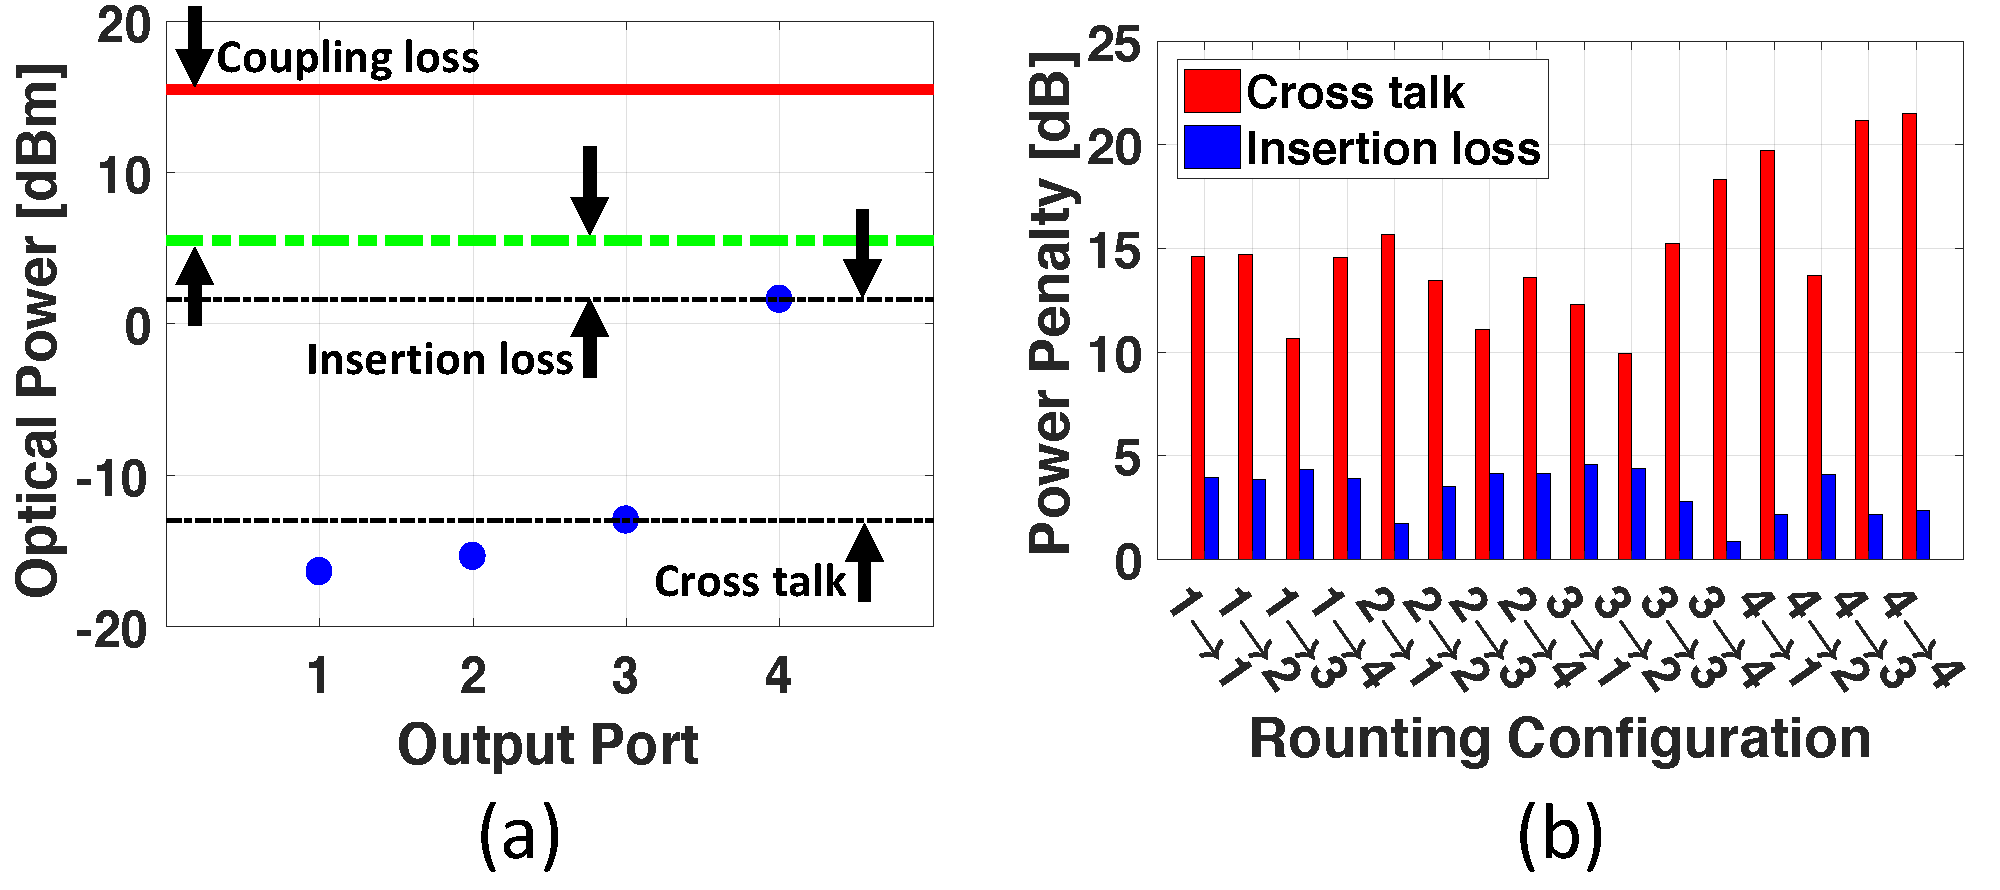
\includegraphics[width=13cm]{Chapter5/fig8_ER_IL3}
\caption{(a) Received optical power measured at all output ports for a single configuration of the switch: input optical data from port 1 to output port 4 (1$\rightarrow$4). The red horizontal line represents the input optical power. The difference to the dashed green line is the loss due to optical fiber coupling. The differences between the green and top dashed black is the insertion loss of switch the and the differences between the top two received optical power represent the cross talk of the configuration. (b) Measured cross talk and insertion loss of all routing configurations of the switch. The x-axis represent the ``input port''$\rightarrow$``output port''.}
\end{figure}

Figure 7(a) shows the measured results for a single routing: 1$\rightarrow$4. Based on the look-up table MZI1-6 are set for the following states [C,-,C,-,B]. The red horizontal line at 15dBm represents the optical input signal operating at 1550nm. 10dB below the laser level, shown in the dashed green line, is the coupling loss. Insertion loss is defined as the loss of the signal due to propagation in the switch in a specific routing configuration. Extinction ratio is the optical power difference between the desired port (port 4) to the second highest level (port 3). For this specific routing the insertion loss is 3.8dB, and the extinction ratio is 14.6dB. 

Similar computations are carried out on the rest of the routing configurations and the results are shown in the bar chart of Fig. 7(b). The crosstalk ranges from 9.92 to 21.51dB and the insertion loss between 0.88--4.59dB. We believe that the variations between the routing performances is caused due to loss variations in the switch such as the couplers and doping level of the heaters. Additionally, due to the small footprint of the $4\times4$ switch (\SI{2000x500 }{\micro\metre}) with vertical and horizontal separation of \SI{250}{\micro\metre} between the $2\times2$ elements, our switch experiences internal thermal crosstalk between the doped-phase shifters when bias voltages are applied simultaneously to the multiple MZIs. 

\subsection{Data transmission}

12.5Gbaud PAM-4 (25Gbps) optical data is used to evaluate the system under transmission conditions, specifically when switching between the routing configurations based on Table 2. Four-level PAM signals, 2$^{15}$ symbols in length, and each containing a training sequence (TS), are generated and loaded into the AWG which was set to operate continuously. After photo-detection at the receive side, the electrical PAM signals are then captured digitally using the RTS. The TS is used both for receiver synchronization and to aid the digital equalization (EQ) process. A Finite Impulse Response (FIR) EQ was used with filter tap weights updated using a decision directed least mean square (DD-LMS) algorithm. EQ, eye-diagram plotting and BER calculations (after PAM demodulation) were performed off-line.

Figure 8(a) shows the collected (oversampled) eye diagrams from the output ports for the 1$\rightarrow$4 routing. The results align with the power levels measured in Fig. 7a. As expected, an open eye is observed at port 4 with a calculated BER of 3.6$\times 10^{-4}$. The next highest optical power is observed in port 3, compared to port 1 and 2, this corresponds to the V{\scriptsize{p-p}} of the measured eyes diagrams. Figure 8(b) summarizes the calculated BERs at the designated output port based on the PC calibrated routing configuration. All the routings exhibit BER performance between 2.7$\times 10^{-4}$ to 5.9$\times 10^{-4}$, which is lower than 7\% overhead hard-decision FEC limit (BER<3.8$\times 10^{-3}$).

\begin{figure}[h!]
\centering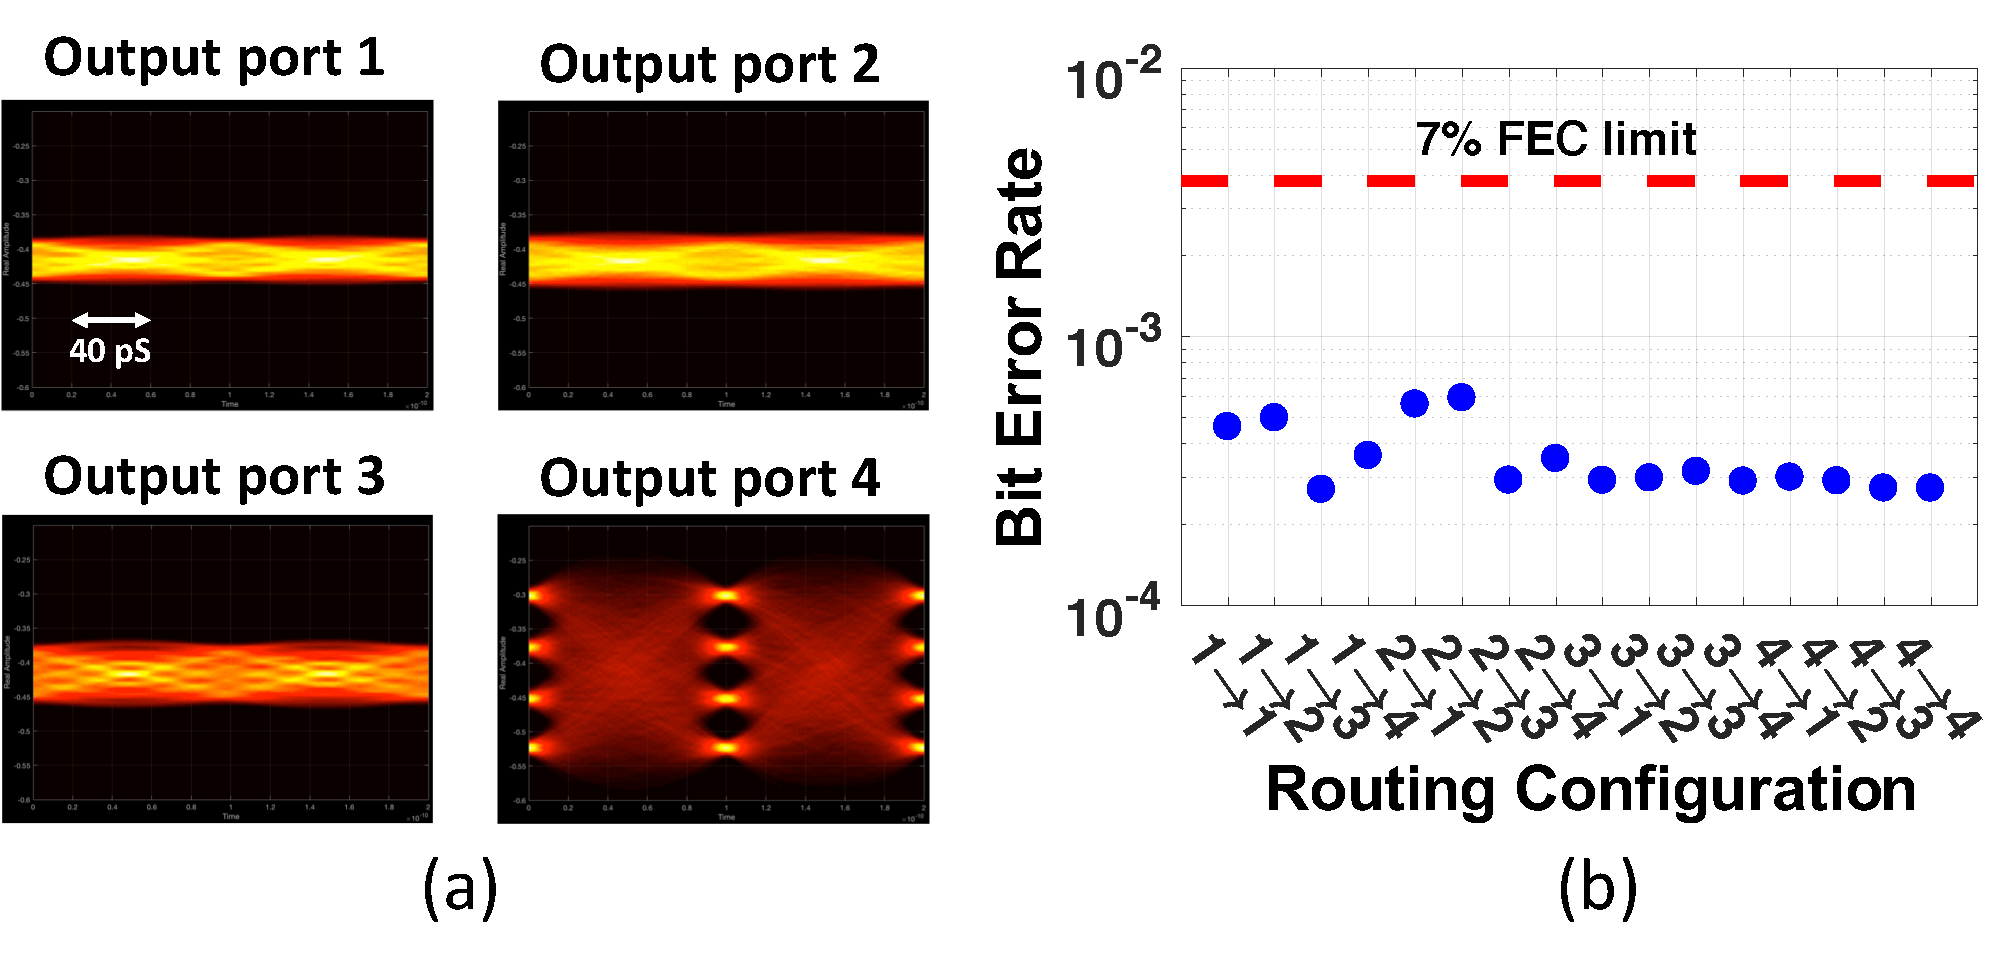
\includegraphics[width=13.5cm]{Chapter5/fig9_eye2}
\caption{Eye diagram results collected at the output ports for a single configuration of the switch: input optical data from port 1 to output port 4 (1$\rightarrow$4). (b) BER results of PAM 25Gbps for all possible routing configurations of the switch. The x-axis represent the ``input port"$\rightarrow$ ``output port".}
\end{figure} 



\section{Conclusion}
%After proofreading the manuscript, compress your .TEX manuscript file and all figures (which should be in EPS format, or PDF format if you are using PDF-\LaTeX) in a ZIP, TAR or TAR-GZIP package. Prism, OSA's article tracking system, will process in \LaTeX mode by default but will use PDF-\LaTeX if PDF figure files are detected. Note: TAR or TAR-GZIP is no longer required. All files must be referenced at the root level (e.g., file \texttt{figure-1.eps}, not \texttt{/myfigs/figure-1.eps}). If there is video or other supplementary materials, the associated files should be uploaded separately.

The use of the PC effect is demonstrated as a topology agnostic solution for calibrating MZI based silicon photonic switches. The steady state and the transient time response is experimentally characterized and analytical models PC current are presented. Based on the effect, a general calibration algorithm that supports cascaded MZI switch designs is outlined. 

The calibration procedure is carried out on a 4$\times$4 Benes design and verified against a more standard procedure using external PD, and is found to operate within a few percent of difference. The calibrated control biases for the cross and bar states are used to reconfigure the switch system for all possible input to output routings. Each configuration is experimentally evaluated for insertion loss (0.88--4.59dB), cross talk (9.92--21.51dB) and BER of 25Gbps PAM4 signals (2.7$\times 10^{-4}$--5.9$\times 10^{-4}$). 

The results prove that the doped phase-shifter heaters can be utilized for both controlling the state of a 2$\times$2 element and as a fast monitoring element of the optical power levels. This provides advantages in terms of saving switch footprint area, reducing design complexity and lower I/O pin count which are important metrics in the design and deployment of scalable photonic switches.
%This is the first chapter of the dissertation

%The following command starts your chapter. If you want different titles used in your ToC and at the top of the page throughout the chapter, you can specify those values here. Since Columbia doesn't want extra information in the headers and footers, the "Top of Page Title" value won't actually appear.
\pagestyle{plain}

\chapter[Silicon Photonic platform for optically connected memory][Top of Page Title]{Title of Chapter 1}

Here you can write some introductory remarks about your chapter.
I like to give each sentence its own line.

When you need a new paragraph, just skip an extra line.

\section{New Section}

By using the asterisk to start a new section, I keep the section from appearing in the table of contents.
If you want your sections to be numbered and to appear in the table of contents, remove the asterisk.


%\pagestyle{plain}

\chapter[Silicon Photonic platform for optically connected memory][Top of Page Title]{Silicon Photonic platform for optically connected memory}

Here you can write some introductory remarks about your chapter.
I like to give each sentence its own line.

When you need a new paragraph, just skip an extra line.

\section{New Section}

By using the asterisk to start a new section, I keep the section from appearing in the table of contents.
If you want your sections to be numbered and to appear in the table of contents, remove the asterisk.


\include{./Conclusion/Conclusion}

%This final section includes your bibliography.

\backmatter

\SingleSpacing %Start single-spacing text before you start the bibliography. We used \bibitemsep earlier in this document to keep bibliography items separated by one line of blank space, but we need to keep the entries themselves single-spaced.
\printbibliography %Print the bibliography. Your bibliography file is defined as Bibliography.bib earlier in this document by the command \addbibresource. It should be kept in the same folder as this file.



\end{document} %All done! Now you're a doctor.
